\chapter{Probabilistic calculations}

\section{Intruder intersection model}\label{sec:intruderIntersectionModel}
\noindent \paragraph{Intruder model} is basically about intersection of 3D objects, because of definition of avoidance grid $\mathscr{A}(t_i)$ most of these methods are numeric. Let us introduce intruder model $\dot{\vec{x}}_I=\vec{f}(\vec{x}_I,\vec{u}_I)$ is given by following equation:
\begin{equation}\label{eq:intruderBasicLinearModel}
    \dot{\vec{x}}_I=
    \begin{aligned}
        \dot{p}_x\\
        \dot{p}_y\\
        \dot{p}_z
    \end{aligned}
    = 
    \begin{aligned}
        =v_x\\
        =v_y\\
        =v_z
    \end{aligned}
    ;\quad
    \vec{x}_I(0)=
    \begin{bmatrix}
        p_x(0)\\
        p_y(0)\\
        p_z(0)
    \end{bmatrix}
    ;\quad
    \begin{aligned}
        p_x(t)\\
        p_y(t)\\
        p_z(t)
    \end{aligned}
    \begin{aligned}
        =p_x(0)+v_x.t\\
        =p_y(0)+v_y.t\\
        =p_z(0)+v_z.t
    \end{aligned}
\end{equation}

\noindent Position vector $[p_x,p_y,p_z]^T$  $(m,m,m\in\R^3$ is given in local coordinate frame of avoidance grid $\mathscr{A}(t_i)$. Velocity vector $[v_x,v_y,v_z]$ $(m.s^{-1},m.s^{-1},m.s^{-1})$ is \emph{estimated and not changing}. The time $t$ is in interval $[t_e,t_l]$, where $t_e$ is intruder entry time into avoidance zone and $t_l$ is intruder leave time from avoidance zone, if vehicle is considered, time of entry is marked as $i_{e,k}$ where k is intruder identification, time of leave is marked as $i_{l,k}$ where k is intruder identification. 

\paragraph{Cell entry and leave times} $t_e(c_{i,j,k})$ and $t_l(c_{i,j,k})$ are given by trajectory $\mathscr{T}(x_0,B)$ and cell space $c_{i,j,k}\in\{x\in\R^3:d_s \le x(1) \le d_e, \theta_s \le x(2) \le \theta_e, \varphi_s \le x(3) \le \varphi_e \}$. From trajectory definition there exist projection $f:\mathscr{T}(x_0,B)\to (\R^3)\times \R$ to avoidance grid coordinate space $x\in \R^3$ and avoidance grid time $t\in\R$. Then intersection of trajectory and cell with time is given as:
\begin{equation}
    (\mathscr{T}(x_0,B)\to (\R^3)\times \R)\cap(c_{i,jk}\times (-\infty,\infty))=\left\{ \vec{x}_e,\dots,\vec{x}_l \right\}\times \left\{ t_e,...,t_l\right\}
\end{equation}
\noindent Where $t_e$ is cell $c_{i,j,k}$ entry time given by function $f_{t_e}(c_{i,j,k},\mathscr{T}(x_0,B))$, $t_l$ is cell leave time given by function $f_{t_l}(c_{i,j,k},\mathscr{T}(x_0,B))$. Entry time $t_e$ and leave time $t_l$ for cell $c_{i,j,k}$ where $\mathscr{T}(c_{i,j,k})$ is set of trajectories are given by eq. (\ref{eq:cellEntryTime}) and (\ref{eq:cellLeaveTime}).
\begin{equation}\label{eq:cellEntryTime}
    t_e=f_{t_e}(c_{i,j,k})=
    \begin{cases}
        -\infty&:|\mathscr{T}(c_{i,j,k})|=0\\
        \min f_{t_e}(c_{i,j,k},\mathscr{T}(x_0,B)),\forall\mathscr{T}(x_0,B)\in \mathscr{T}(c_{i,j,k})&:|\mathscr{T}(c_{i,j,k})|\neq 0\\
    \end{cases}
\end{equation}

\begin{equation}\label{eq:cellLeaveTime}
    t_l=f_{t_l}(c_{i,j,k})=
    \begin{cases}
        \infty&:|\mathscr{T}(c_{i,j,k})|=0\\
        \max f_{t_l}(c_{i,j,k},\mathscr{T}(x_0,B)),\forall\mathscr{T}(x_0,B)\in \mathscr{T}(c_{i,j,k})&:|\mathscr{T}(c_{i,j,k})|\neq 0\\
    \end{cases}
\end{equation}

\paragraph{Intruder intersection probability} $P_{O_I}(i_k)$ for intruder $i_k$ intersection with vehicle in cell $c_{i,j,k}$ is given by eq. (\ref{eq:intruderIntersectionProbability}).
\begin{equation}\label{eq:intruderIntersectionProbability}
    P_{O_I}(i_k)=\frac{\norm{[i_e(c_{i,j,k}),i_l(c_{i,j,k})]\cap [t_e,t_l]}}{\norm{[t_e,t_l]}}.P_T(i_k,c_{i,j,k})
\end{equation}
\noindent Base intersection probability $P_T(i_k,c_{i,j,k})$ shows how probable is to meet intruder $i_k$ in cell $c_{i,j,k}$, enumerator $\norm{[i_e(c_{i,j,k}),i_l(c_{i,j,k})]\cap [t_e,t_l]}$ represents time duration which intruder $i_k$ and our vehicle spends together in cell $c_{i,jk}$, where $i_e$ is intruder entry, $i_l$ is intruder leave, $t_e$ is vehicle entry, $t_l$ is vehicle leave, denominator $\norm{[t_e,t_l]}$ is maximum duration of vehicle passing trough cell $c_{i,j,k}$. \textit{The main principle} is to calculate probability of staying in same portion of space for vehicle and intruder $i_k$. In case the numeric approximation is used and the result is set of intersection times/position pairs $\{(t_1,\vec{p}_1),\dots,(t_k,\vec{p}_k)\}$ where position set $\{\vec{p}_1,\dots,\vec{p}_k\}\in c_{i,j,k}$  then (\ref{eq:intruderIntersectionProbability}) is re-written as:
\begin{equation}\label{eq:intruderIntersectionProbabilityNumeric}
    P_{O_I}(i_k)=\frac{|\{t_1,\dots,t_k\}\cap [t_e,t_l]|}{k}.P_T(i_k,c_{i,j,k}),\quad \{t_1,\dots,t_k\},k\in \N^+
\end{equation}
\noindent Base intersection probability $P_T(i_k,c_{i,j,k})$  stays same it is not impacted. The time intersection probability is calculated differently, enumerator  $|\{t_1,\dots,t_k\}\cap [t_e,t_l]|$ is resulting into count of how many numeric hits landed vehicle entry/leave interval $[t_e,t_l]$. Denominator is simple count of hits which landed into cell $c_i,j,k$. The final ratio shows how probable is to encounter intruder $i_k$ in cell $c_{i,j,k}$. The principle of (\ref{eq:intruderIntersectionProbabilityNumeric}) is same as (\ref{eq:intruderIntersectionProbability})  but instead of interval intersection, set intersection is used.

\paragraph{Base intersection probability} $P_T(i_k,c_{i,j,k})$ reflects probability of vehicle intersection with portion of space occupied by cell $c_{i,j,k}$, to be precise with vehicle trajectory or vehicle body shifted among that trajectory. This work considers two trajectories representation:
\begin{enumerate}
    \item \textit{Direct line} - vehicle trajectory is represented as basic linear model (\ref{eq:intruderBasicLinearModel}), depending on average cell volume and safety margin condition direct line can have two intersection modes:
    \begin{enumerate}[a.]
        \item \textit{simple line} - intersection is approximated along line defined by intruder model (\ref{eq:intruderBasicLinearModel}).
        \item \textit{volume line} - intersection is approximated along line defined by intruder model (\ref{eq:intruderBasicLinearModel}) and intruder radius $r_i$ $[m]$ is considered in intersection.
    \end{enumerate}
    \item \textit{Elliptic cone} - initial position $\vec{x}_i(0)$ is considered as top of the cone, main cone axis is given by line (\ref{eq:intruderBasicLinearModel}) $t\in [-\infty,\infty]$. The cone is defined by horizontal spread parameter $\theta$ and vertical spread $\varphi$.
\end{enumerate}

\paragraph{Base intersection probability - simple line type} $P_T(i_k(\vec{x},\vec{v}),c_{i,j,k})$ is simple linear intersection with line defined as expected intruder $i_r$ trajectory (\ref{eq:linearModelIntruderLineIntersection}). Intruder trajectory is defined by starting point $\vec{x}_s\in\R^3$ and linear velocity vector $\vec{v}\in\R^3$. 
\begin{equation}\label{eq:linearModelIntruderLineIntersection}
    \vec{x}(t)=\vec{x}_s + \vec{v}_I.t
\end{equation}
\noindent Then there exist projection function from local euclidean coordinates to local planar coordinates $p(t)$ (\ref{eq:projecionFunctionplanarEuclidlinearIntersection}). Which projects trajectory of the system $\vec{x}(t)\in\R^3$ to planar coordinates $[d(t),\theta(t),\varphi(t)]$. Where $d$ is distance, $\theta$ is horizontal offset angle from main axis, and $\varphi$ is vertical offset angle from main axis.
\begin{equation}\label{eq:projecionFunctionplanarEuclidlinearIntersection}
    \vec{p}(t):\vec{x}(t)\to[d(t),\theta(t),\varphi(t)]
\end{equation}
\noindent The \emph{base intersection probability} $P_T(i_k(\vec{x},\vec{v}),c_{i,j,k})$ for line type is given as eq. \ref{eq:baseIntersectionProbabilityLineIntersectionType}. If there exist non empty intersection of $p(t)\cap c_{i,j,k}$ there is direct collision probability, if intersection $p(t)\cap c_{i,j,k} = \varnothing$ then probability is zero.
\begin{equation}\label{eq:baseIntersectionProbabilityLineIntersectionType}
    P_T(i_k(\vec{x},\vec{v}),c_{i,j,k})=
    \begin{cases}
        1&\exists d(t),\theta(t),\varphi(t),[d(t),\theta(t),\varphi(t)]^T\in c_{i,j,k}\\
        0&\text{otherwise}
    \end{cases}
\end{equation}

\paragraph{Base intersection probability - volume line type} $P_T(i_k(\vec{x},\vec{v},r),c_{i,j,k})$ is defined for linear intersection model $\vec{x}(t)$ (\ref{eq:linearintersectionmodelVehicleVolume}) where initial position $\vec{x}_s$ is given at expected time of avoidance $t_i$ in avoidance grid $\mathscr{A}(t_i)$ local coordinate frame, velocity vector $\vec{v}$ is given in same reference frame.
\begin{equation}\label{eq:linearintersectionmodelVehicleVolume}
    \vec{x}(t)=\vec{x}_s + \vec{v}.t
\end{equation}

\noindent\emph{Volume ball} $\mathscr{B}(\vec{x}(t),r)$ (\ref{eq:volumeballofIntruder}) is defined as set of points in $\R^3$ space with defined center at intruder $i_r$ position $\vec{x}(t)$. The inclusion criterion is set to a full ball. Volume ball $\mathscr{B}(\vec{x}(t),r)$ represents approximation of vehicle body expected position at time $t$.
\begin{equation}\label{eq:volumeballofIntruder}
    \mathscr{B}(\vec{x}(t),r)= \left\{\vec{a}\in\R^3:\exists t,\norm{\vec{a}-\vec{x}(t)}_2\le r\right\}
\end{equation}

\noindent\emph{Planar volume ball} $\mathscr{P}_\mathscr{B}$ (\ref{eq:plannarCoordinateTransformationVolumeBall}) is projection of volume ball $\mathscr{B}(\vec{x}(t))$ to a set of planar coordinates $\left\{[d,\theta,\varphi]\right\}$ in avoidance grid $\mathscr{A}(t_i)$ local coordinate frame for expected avoidance time $t_i$.
\begin{equation}\label{eq:plannarCoordinateTransformationVolumeBall}
    \mathscr{P}_\mathscr{B}=\mathscr{B}(\vec{x}(t),r)\to \left\{[d,\theta,\varphi]\right\}
\end{equation}

\noindent\emph{Base intersection probability for vehicle body} $P_T(i_k(\vec{x},\vec{v},r),c_{i,j,k})$ \ref{eq:baseIntersectionProbabilityBallIntersectionType} is calculated as intersection of planar volume ball $\mathscr{P}_\mathscr{B}$ and cell $c_{i,j,k}$. If intersection $\mathscr{P}_\mathscr{B}\cap c_{i,j,k} \neq \varnothing$ is non empty then base probability is one, zero otherwise.
\begin{equation}\label{eq:baseIntersectionProbabilityBallIntersectionType}
    P_T(i_k(\vec{x},\vec{v},r),c_{i,j,k})=
    \begin{cases}
        1&\mathscr{P}_\mathscr{B}\cap c_{i,j,k} \neq \varnothing\\
        0&\text{otherwise}
    \end{cases}
\end{equation}

\paragraph{Base intersection probability - elliptic cone type} $P_T(i_k(\vec{x}_s,\vec{v},\theta,\varphi),c_{i,j,k})$
computation is less straight-forward than other base intersection probabilities. First let us define linear intruder $i_k$ positions $\vec{x}$ at time $t$ (\ref{eq:vehiclelinearcone}) model, where $\vec{x}(t)$ defines vehicle position in \emph{vehicle local coordinate frame} at time of avoidance, $\vec{v}$ defines intruder velocity, and $t$ is time offset.
\begin{equation}\label{eq:vehiclelinearcone}
    \vec{x}(t)=\vec{x}_s + \vec{v}_I.t
\end{equation}
\noindent Intruder \emph{horizontal spread} $\theta$ and \emph{vertical spread} $\varphi$ are introduced. These spreads represents intruder deviation limits from original trajectory $\vec{x}(t)\in\R^3$. The example is given by fig. \ref{fig:P21ElipticConeIOnePoint} where intruder starts at point $\vec{x}_s$ with some velocity $v$, the linear trajectory approximation is given by blue line. \emph{Intruder position} at time $t=10s$ is given by $\vec{x}(10)$ and is denoted blue point. The ellipsoidal space $E(\vec{x})$ is projected on plane $D(\vec{x}(t))$. The plane $D$ (\ref{eq:elisioidalOtrthogonalPlane}) for point $\vec{x}(t)$ and velocity $\vec{v}$ is defined as orthogonal plane to velocity $\vec{v}\in\R^3$ with origin at intruder position $\vec{x}(t)$. 
\begin{equation}\label{eq:elisioidalOtrthogonalPlane}
    D(\vec{x}(t),\vec{v})=\left\{\vec{a}\in\R^3:(\vec{a}-\vec{x}(t))\perp\vec{v},\right\}
\end{equation}
\noindent To introduce ellipsoidal space on orthogonal plane $D(\vec{x}(t),\vec{v})$ some parameters are introduced in eq. (\ref{eq:elipsiodialBoudaryParameters}). The \emph{scalar distance} $d_d{\vec{x}(t)}$ is simple euclidean norm, \emph{maximal horizontal offset} $d_\theta(\vec{x}_t)$ is given as product of sinus of horizontal offset angle $\theta$ and scalar distance $d_d$, and \emph{maximal vertical offset} $d_\varphi(\vec{x}(t))$ is given a product of sinus of vertical offset angle $\varphi$ and scalar distance $d_d$.
\begin{equation}\label{eq:elipsiodialBoudaryParameters}
    \begin{aligned}
     d_d                      &=d_d(\vec{x}(t),\vec{x}_s) =\norm{\vec{x}(t)-\vec{x}_s}_2\\ 
     d_{\theta_{\text{max}}}  &= d_\theta(\vec{x}(t))=\sin\theta   (i_k).d_d(\vec{x}(t))\\
     d_{\varphi_{\text{max}}} &= d_\varphi(\vec{x}(t))=\sin\varphi (i_k).d_d(\vec{x}(t)) 
    \end{aligned}
\end{equation}
\begin{figure}[H]
    \centering
    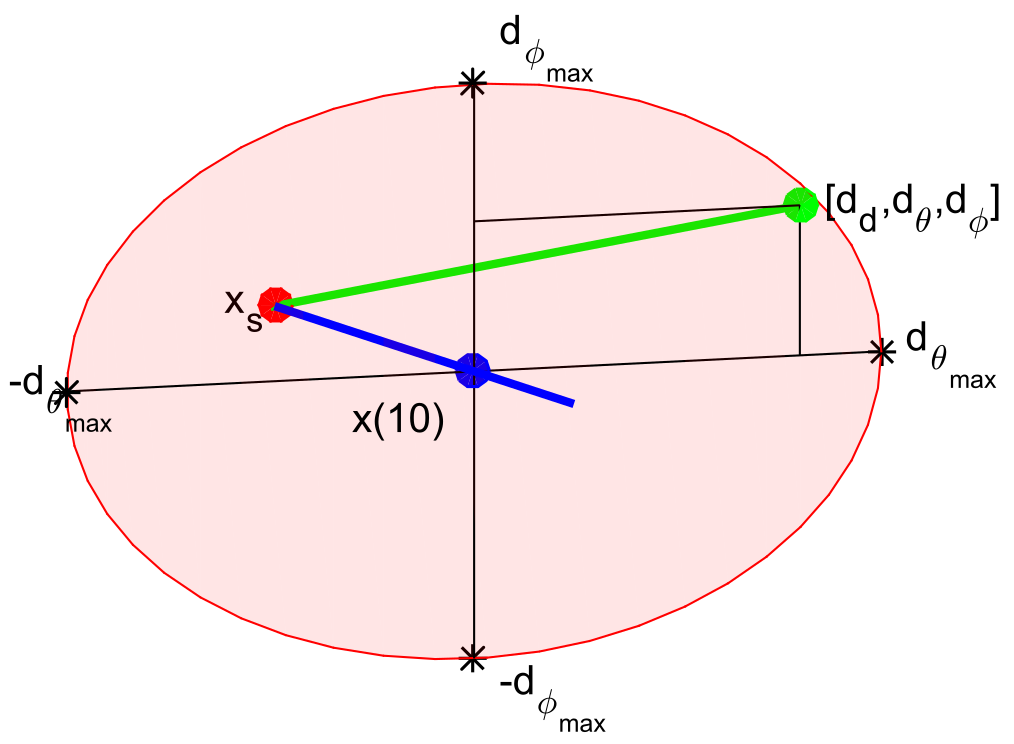
\includegraphics[width=0.7\textwidth]{\FIGDIR/P21ElipticConeIOnePoint}
    \caption{One probable position $[d_d,d_\theta,d_\varphi]$ (green). deviated from linear trajectory (blue line) at point $\vec{x}(10)$.(blue) with initial position $x_s$ (red)}
    \label{fig:P21ElipticConeIOnePoint}
\end{figure}
\noindent \emph{Ellipsoid} $E(\vec{x}(t),\vec{v})$ (\ref{eq:baseElipsoidxt}) for some intruder position $\vec{x}(t)$ and intruder velocity $\vec{v}$ is given as constrained subspace of orthogonal plane $D(\vec{x}(t),\vec{v})$. The constraint is defined by internal coordinate frame $\vec{p}\in \R^2$ which is space reduction of plane $D(\vec{x}(t),\vec{v})$. Internal coordinate frame $\vec{p}\in\R^2$ has origin in $\vec{x}(t)\to\R^2$. The points of plane $\vec{p}$ are bounded by projection $\vec{p}=(\vec{b}-\vec{x}(t))\to\R^2$, where $b\in D(\vec{x}(t),v)$. The point of ellipsoidal $\vec{p}$ is then given as standard ellipse boundary with vertical span $d_\theta(\vec{x}(t))$ and horizontal span $d_\varphi(\vec{x}(t))$. \emph{Ellipsoid} $E(\vec{x}(t),\vec{v})$ for specific time $t=10s$ example is portrayed  as red elipsoind in fig. \ref{fig:P21ElipticConeIOnePoint}.
\begin{equation}\label{eq:baseElipsoidxt}
    E(\vec{x}(t),\vec{v})=\left\{ \begin{aligned}\vec{b}\in\R^3:&\vec{b}\in D(\vec{x}(t),\vec{v}),\vec{p}=(\vec{b}-\vec{x}(t))\to\R^2,\\&\left(\frac{p(1)^2} {d_\theta(\vec{x}(t))^2}+ \frac{p(2)^2}{d_\varphi(\vec{x}(t))^2}\right)\le 1\end{aligned}\right\}
\end{equation}

\noindent The expected behaviour of intruder $i_k$ is to stick to linear trajectory $\vec{x}(t)$ (\ref{eq:vehiclelinearcone}). The probability of deviation should be decreasing with distance from ellipse center (fig. \ref{fig:P22ProbabilisticDistributionOfEllipsoidCut}.).  
\begin{figure}[H]
    \centering
    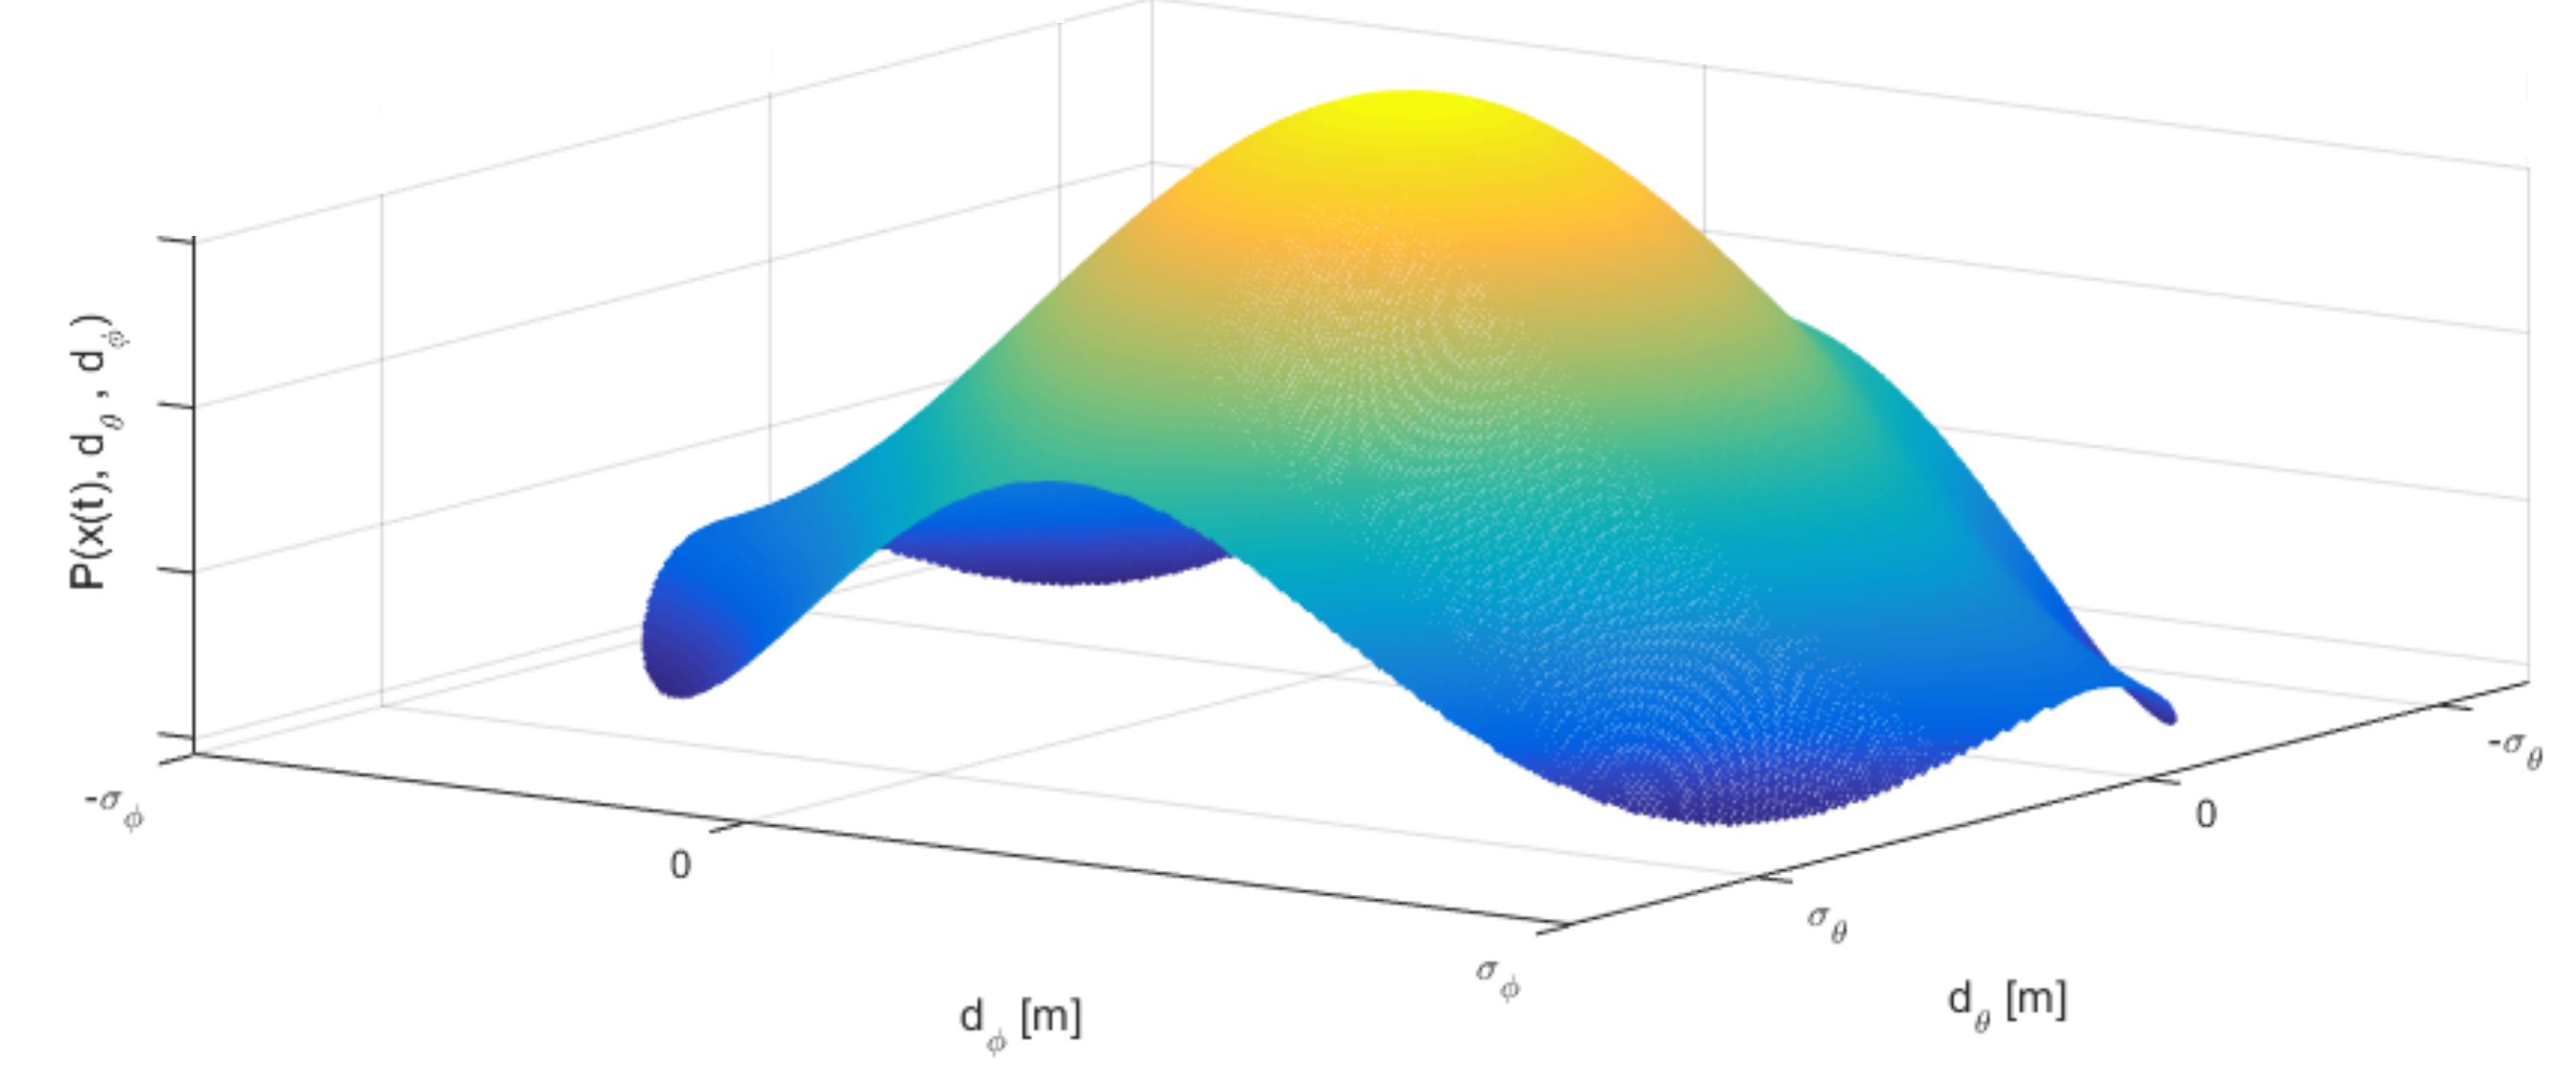
\includegraphics[width=0.9\textwidth]{\FIGDIR/P22ProbabilisticDistributionOfEllipsoidCut}
    \caption{Probability of intruder $i_k$ position in ellipsoid $E(\vec{x}(t),\vec{v})$}
    \label{fig:P22ProbabilisticDistributionOfEllipsoidCut}
\end{figure}
\noindent \emph{Probability density function} for ellipsoid  $E(\vec{x}(t),\vec{v})$defined in (\ref{eq:baseElipsoidxt}) is depending on maximal horizontal spread $d_\theta(\vec{x}(t))$, maximal vertical spread $d_\varphi(\vec{x}(t))$, defined by eq. \ref{eq:elipsiodialBoudaryParameters}. Two standard probabilistic distributions are established $\mathscr{N}(\mu_\theta,\sigma_\theta)$ (\ref{eq:elipsprobdistHorizontal}) for horizontal spread $\theta(\vec{x}(t))$ and $\mathscr{N}(\mu_\varphi,\sigma_\varphi)$  (\ref{eq:elipsprobdistVertical}) for vertical spread $\varphi(\vec{x}(t))$. The means $\mu_\theta$ and $\mu_\varphi$ are set to zero, and internal coordinate frame $\vec{p}\in\R^2$ where $\vec{x}(t)\to\R^2$ is frame center. The variances $\sigma_\theta$ and $\sigma_\varphi$ are set as maximal distances on horizontal/vertical spread axes $d_\theta(\vec{x}(t))$ and $d_\varphi(\vec{x}(t))$.
\begin{equation}\label{eq:elipsprobdistHorizontal}
    P(\vec{x}(t),d_\theta)=\mathscr{N}(\mu_\theta,\sigma_\theta)=\mathscr{N}(0,d_\theta(\vec{x}(t)))
\end{equation}
\begin{equation}\label{eq:elipsprobdistVertical}
    P(\vec{x}(t),d_\varphi)=\mathscr{N}(\mu_\varphi,\sigma_\varphi)=\mathscr{N}(0,d_\varphi(\vec{x}(t)))
\end{equation}
\noindent Combined \emph{probability density function} for maximal spreads $d_\theta$ and $d_\varphi$ is given by eq. \ref{eq:elipsprobdistCombined}. Because probability density function is defined for internal space $\vec{p}\in\R^2$ and one may need to calculate probability for for cell space $c_{i,j,k}\in\R^3$, the reduction from two parameter probability distribution function to scalar probability distribution function is needed. Scalar probabilistic distribution  function $P(\vec{x}(t),d_\theta,d_\varphi)$ over ellipsoid $E(\vec{x}(t),\vec{v})$ is introduced (\ref{eq:elipsprobdistCombined}), where final probability is given as average of two partial probabilities. Final $P(\vec{x}(t),d_\theta,d_\varphi)$ needs to be normalized to hold \emph{normal distribution condition} (\ref{eq:normalDistrobitionCondition}). Normal distribution condition value (\ref{eq:normalDistrobitionCondition}) is given as surface integral over ellipsoid $E(\vec{x}(0),\vec{v})$ with probability density function $P(\vec{x}(t),d_\theta,d_\varphi)$.
\begin{equation}\label{eq:elipsprobdistCombined}
    P(\vec{x}(t),d_\theta,d_\varphi) = \frac{\mathscr{N}(\mu_\theta,\sigma_\theta)+\mathscr{N}(\mu_\varphi,\sigma_\varphi)}{2}
\end{equation}
\begin{equation}\label{eq:normalDistrobitionCondition}
    \iint_{E(\vec{x}(\tau))} P(\vec{x}(t),d_\theta,d_\varphi) \,\text{d}d_\theta\,\text{d}d_\varphi = 1
\end{equation}
\noindent Final intersection probability  $P(\vec{x}(t),c_{i,j,k},\theta,\varphi)$ (static part, timed is calculated in (\ref{eq:intruderIntersectionProbability}) is given by eq. \ref{eq:spreadIntruderIntersectionProb}. Its mean value of all intersection probabilities $P(\vec{x}(\tau),c_{i,j,k},\theta,\varphi)$ where $\tau\in[i_e(c_{i,j,k}),i_l(c_{i,j,k})]$ is fixed point in intersection time interval. $P(\vec{x}(\tau),c_{i,j,k},\theta,\varphi)$ (\ref{eq:spreadIntersectionProbFixedtau}) is integration of probability density function $P(\vec{x}(\tau),d_\theta,d_\varphi)$ (\ref{eq:elipsprobdistCombined}) in surface $E(\vec{x}(\tau),\vec{v})$ to cell $c_{i,j,k}$ volume intersection. To get volume integration partial probability in surface intersection must be integrated and normalized in time interval $\tau\in[i_e(c_{i,j,k}),i_l(c_{i,j,k})]$, the \emph{base intersection probability} $P_T(i_k(\vec{x}_s,\vec{v},\theta,\varphi),c_{i,j,k})$ is given by eq. \ref{eq:spreadIntruderIntersectionProb}. Example of intersection of intruder $i_r$ uncertain ellipsoid cone with avoidance grid $\mathscr{A}(t_i)$ is given in fig. \ref{fig:P20ElipticConeIntersecitonExample}.
\begin{equation}\label{eq:spreadIntersectionProbFixedtau}
    P(\vec{x}(\tau),c_{i,j,k},\theta,\varphi) =\iint_{E(\vec{x}(\tau),\vec{v})\cap c_{i,j,k}} P(\vec{x}(\tau),d_\theta,d_\varphi)
\end{equation}
\begin{equation}\label{eq:spreadIntruderIntersectionProb}
    P_T(i_k(\vec{x}_s,\vec{v},\theta,\varphi),c_{i,j,k})=\frac{\int_{i_e(c_{i,j,k})}^{i_l(c_{i,j,k})} P(\vec{x}(\tau),c_{i,j,k},\theta,\varphi)\,\text{d}\tau}{i_l(c_{i,j,k})-i_e(c_{i,j,k})}
\end{equation}
\begin{figure}[H]
    \centering
    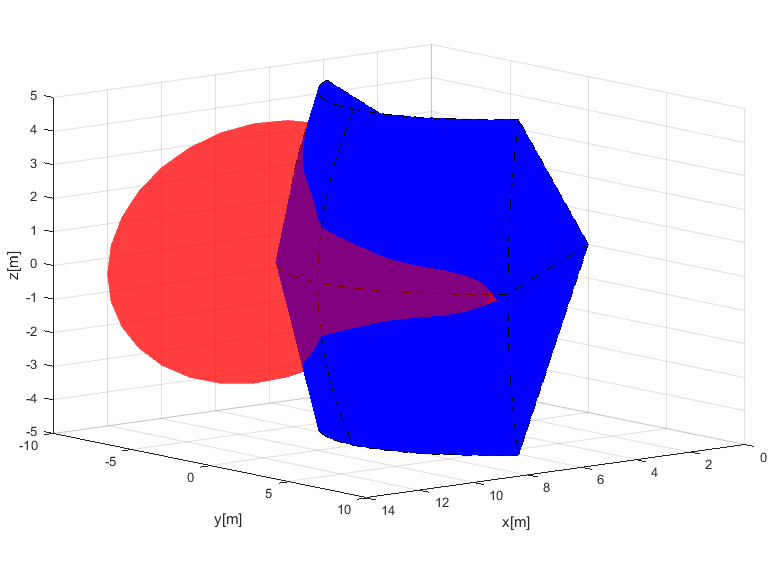
\includegraphics[width=0.7\textwidth]{\FIGDIR/P20ElipticConeIntersecitonExample}
    \caption{Avoidance grid $\mathscr{A}(t_i)$ (blue) intersection with elliptic cone intruder $i_k(\vec{x},\vec{v},\theta,\varphi)$ (red) example.}
    \label{fig:P20ElipticConeIntersecitonExample}
\end{figure}
\noindent \emph{Numeric approximation} of $P_T(i_k(\vec{x}_s,\vec{v},\theta,\varphi),c_{i,j,k})$ is more feasible than symbolic calculation due the multiple intersection constraints and bad intersection algorithm complexity. Let us define homogeneous discrete subset of real numbers $\mathscr{R}$ which is non empty subset of real numbers $\R$. The set $\mathscr{R}$ (\ref{eq:homogeneusdiscretizationofRealnumbers}) is homogeneous, that means for any equal interval $(i,i+1],i\in\mathbb{Z}$ subset the count of members is equal to some positive natural number $k$. The parameter $k$ can be understand as \emph{unit approximation density}.
Similarly the power sets $\mathscr{R}^2\subset\R^2$, $\mathscr{R}^3\subset\R^3$, ... $\mathscr{R}^i\subset\R^i,i\in\N^+$ keeps homogeneous distribution.
\begin{equation}\label{eq:homogeneusdiscretizationofRealnumbers}
    \mathscr{R} = \left\{\begin{aligned}a\in\R:&\forall i\in\mathbb{Z},|i<a\le i+1|=k,k\in\N^+, \\&\forall j\in \N^+a_{j+1}-a_{j}=m,m\in\R^+\end{aligned}\right\},\,\mathscr{R}\subset\mathbb{R}
\end{equation}
\noindent Orthogonal plane for $\vec{x}(t), \vec{v}, t \in\R$ is defined by eq. \ref{eq:elisioidalOtrthogonalPlane}. The orthogonality property is also kept for any subspace $\mathscr{R}^n\in\R^n,n\in\N^+$. Numeric approximation of $D(\vec{x}(t),\vec{v})$ is given as $D_D(\vec{x}(t),\vec{v})$ (\ref{eq:elisioidalOtrthogonalPlaneDiscrete}). The only difference is that discrete approximation is countable $|D_D|=m,m\in\N^+$, but continuous representation $|D|\approx \infty$ is uncountable. Because ellipsoid is subset of orthogonal plane it keep its countability property, therefore $E_D$ is also countable and must contains at-least one member.  
\begin{equation}\label{eq:elisioidalOtrthogonalPlaneDiscrete}
    D_D(\vec{x}(t),\vec{v})=\left\{\vec{a}\in\mathscr{R}^3:(\vec{a}-\vec{x}(t))\perp\vec{v},\right\},t\in\mathscr{R}
\end{equation}
\noindent\emph{Base ellipsoid} $E(\vec{x}(t),\vec{v})$ for continuous-space is given by eq. \ref{eq:baseElipsoidxt}. Every aspect, expect the base of internal projection $\mathscr{R}^2$ and orthogonal plane $D_D$ is same in discrete case $E_D(\vec{x}(t),\vec{v})$ (\ref{eq:baseElipsoidxtDiscrete}).
\begin{equation}\label{eq:baseElipsoidxtDiscrete}
    \bar{E}_D(\vec{x}(t),\vec{v})=\left\{ \begin{aligned}\vec{b}\in\mathscr{R}^3:&\vec{b}\in D_D(\vec{x}(t),\vec{v}),\vec{p}=(\vec{b}-\vec{x}(t))\to\mathscr{R}^2,\\&\left(\frac{p(1)^2} {d_\theta(\vec{x}(t))^2}+ \frac{p(2)^2}{d_\varphi(\vec{x}(t))^2}\right)\le 1\end{aligned}\right\},t\in\mathscr{R}
\end{equation}
\noindent \emph{Numeric disproportion} can occur in case that ellipsoid $\bar{E}_D(\vec{x}(t),\vec{v})$ (\ref{eq:baseElipsoidxtDiscrete}) in case of $d_\theta(\vec{x}(t))\approx 0$ and $d_\varphi(\vec{x}(t))\approx 0$. The count of elipsoid members can be $|\bar{E}_D(\vec{x}(t),\vec{v})|=0$, which is in contradiction with assumption $|\bar{E}_D(\vec{x}(t),\vec{v})|\neq 0$. Let assume for discrete times $\tau=\left\{t_1,t_2,\dots,t_i\right\}$, $i\in \N^+$ there exists ellipsoids $\bar{E}_D(\vec{x}(t_1),\vec{v})$,$\bar{E}_D(\vec{x}(t_1),\vec{v})$, $\dots$, $\bar{E}_D(\vec{x}(t_i),\vec{v})$ which are non empty and in space $\mathscr{R}^2$ in internal coordinate frame and space $\mathscr{R}^3$ in avoidance grid $\mathscr{A}(t_i)$ coordinate frame. The intersection of these partial ellipsoids in both spaces is equal to:
\begin{equation}
    \bar{E}_D(\vec{x}(t_1),\vec{v})\cap \bar{E}_D(\vec{x}(t_2),\vec{v})\dots\cap\dots \bar{E}_D(\vec{x}(t_i),\vec{v}) = \varnothing
\end{equation}
\noindent \emph{Empty intersection} enables us to keep homogeneity property of ellipsoids by adding points so it is safe to add specific point $\vec{x}(t)$ into empty ellipsoid. But only one, because it does not impact probability density functions $\mathscr{N}(\mu_\theta,\sigma_\theta)$ and $\mathscr{N}(\mu_\varphi,\sigma_\varphi)$, neither combined probability density function $P(\vec{x},d_\theta,d_\varphi)$. The final ellipsoid used forward $E_D(\vec{x}(t),\vec{v})$(\ref{eq:baseElipsoidxtDiscreteSafe}) is keeping all properties of ellipsoid $E(\vec{x}(t),\vec{v})$ (\ref{eq:baseElipsoidxtDiscreteSafe}). 
\begin{equation}\label{eq:baseElipsoidxtDiscreteSafe}
    E_D(\vec{x}(t),\vec{v})= 
    \begin{cases}
        |\bar{E}_D(\vec{x}(t),\vec{v})|=0 &: \left\{\vec{x}(t)\right\} \\
        |\bar{E}_D(\vec{x}(t),\vec{v})|\ge0 &: \bar{E}_D(\vec{x}(t),\vec{v}) 
    \end{cases}
\end{equation}
\noindent Normal distribution condition for probability function $P_D(\vec{x}(t),d_\theta,d_\varphi,\vec{p})$, which is instance of to probability density function $P(\vec{x}(y),d_\theta,d_\varphi)$ (\ref{eq:elipsprobdistCombined}) is used. This probabilistic distribution must be normalized according to eq.  \ref{eq:normalDistrobitionConditionDiscrete}. 
\begin{equation}\label{eq:normalDistrobitionConditionDiscrete}
    \sum_{\vec{p} \in E_D(\vec{x}(t))} P_D(\vec{x}(t),d_\theta,d_\varphi,\vec{p}) = 1,\forall t\in\mathscr{R}^+
\end{equation}
\noindent Equations for \emph{base intersection probability} are similar to eq. \ref{eq:spreadIntersectionProbFixedtau}, \ref{eq:spreadIntruderIntersectionProb}. For cell $c_{i,j,k}$ there exist intruder entry time $i_e(c_{i,j,k})$ its the earliest intersection with ellipsoid $E_D(\vec{x}(i_e(c_{i,j,k}))),\vec{v}$. Same situation occurs with intruder leave time $i_l(c_i,j,k)$. Because $E_D$ is countable set, it means additional attributes can be attached to each point $\vec{p}\in E_D$. Based on system dynamic (\ref{eq:intruderBasicLinearModel}) the \emph{Time Of Arrival} (TOA) can be calculated. The example of TOA is given in fig. \ref{fig:P23EllipsoidCutTimeOfArrival}.
\begin{figure}[H]
    \centering
    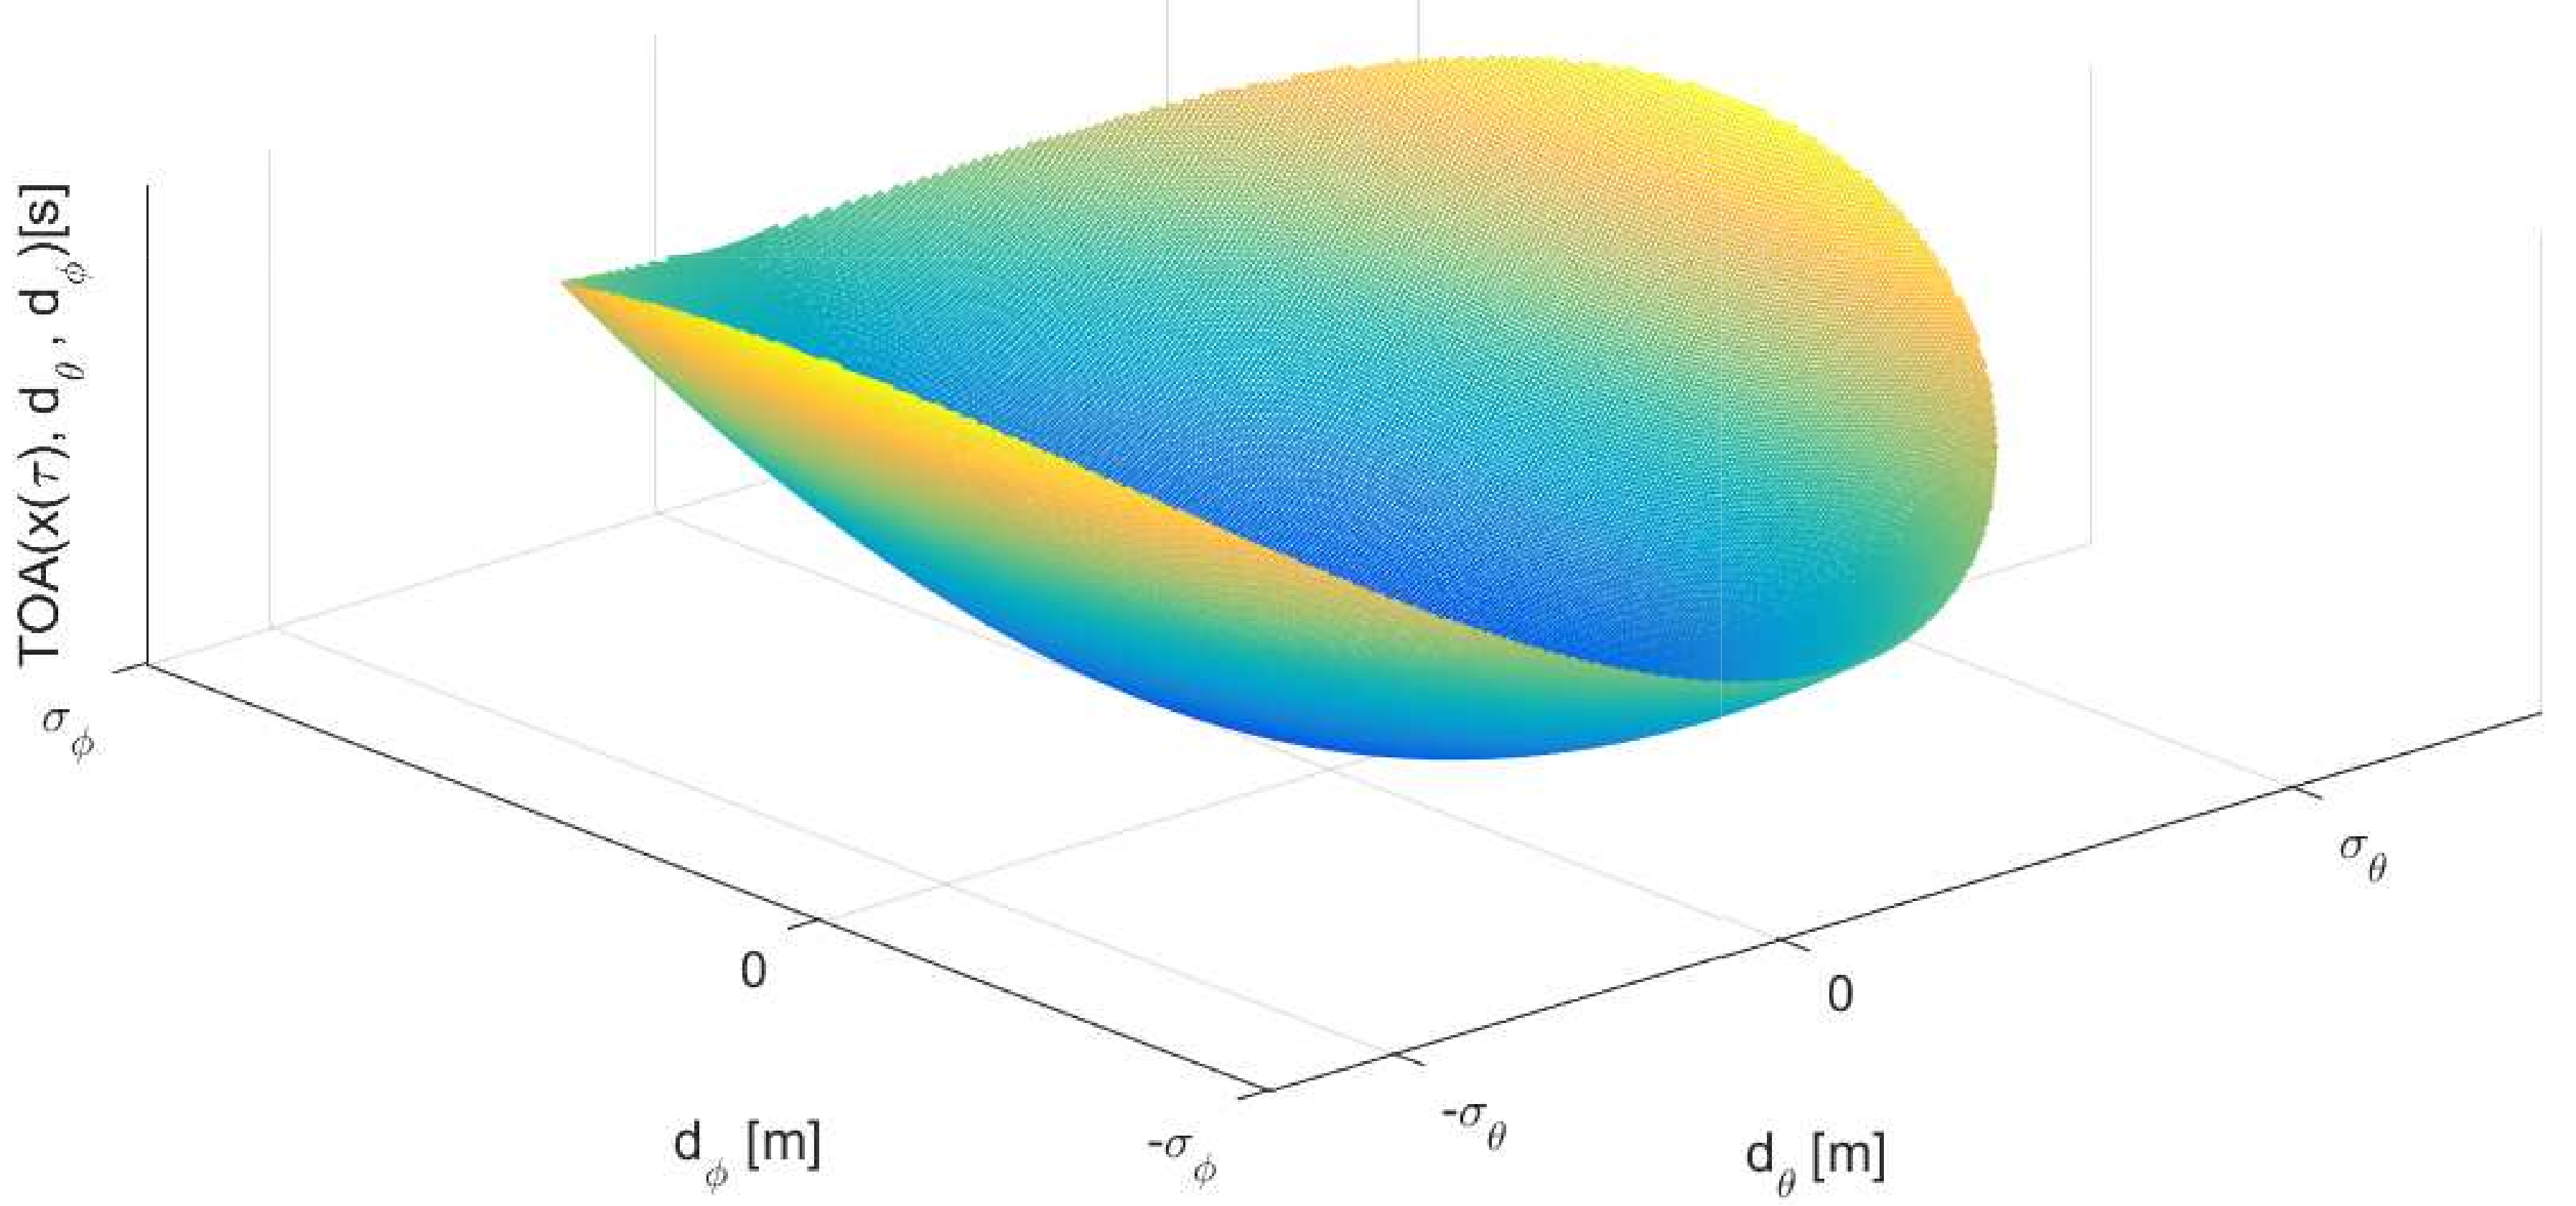
\includegraphics[width=0.7\textwidth]{\FIGDIR/P23EllipsoidCutTimeOfArrival}
    \caption{Time Of Arrival (TOA) for one ellipsoid $E_D(\vec{x}(\tau),\vec{v})$}
    \label{fig:P23EllipsoidCutTimeOfArrival}
\end{figure}
\noindent The intersection probability $P_D(\vec{x}(\tau),c_{i,j,k},\theta,\varphi)$ for one time sample $\tau$ is given by eq. \ref{eq:spreadIntersectionProbFixedtauDiscrete}, which has similar notation to eq. \ref{eq:spreadIntersectionProbFixedtau}, sums are used instead of integrals and discrete probability density function $P_D(\vec{x}(\tau),d_\theta,d_\varphi,\vec{p})$ for points form elipse and cell intersection are used as iterator base set $\vec{p}\in\left\{E_D(\vec{x}(\tau),\vec{v})\cap c_{i,j,k}\right\}$.
\begin{equation}\label{eq:spreadIntersectionProbFixedtauDiscrete}
    P_D(\vec{x}(\tau),c_{i,j,k},\theta,\varphi) =\sum_{\vec{p}\in \left\{E_D(\vec{x}(\tau),\vec{v})\cap c_{i,j,k}\right\}} P_D(\vec{x}(\tau),d_\theta,d_\varphi,\vec{p})
\end{equation}
\noindent The \emph{base intersection probability} $P_{TD}(i_k(\vec{x}_s,\vec{v},\theta,\varphi),c_{i,j,k})$ \ref{eq:spreadIntruderIntersectionProbDiscrete} is given as mean intersection probability of partial intersections $P_D(\vec{x}(\tau),c_{i,j,k},\theta,\varphi)$ where step set $T=\{$ $i_e(c_{i,j,k})$, $\dots$, $i_l(c_{i,j,k})\}$ contains all viable intersection times with ellipsoids $E(\vec{x}(\tau\in T),\vec{v})$. The denominator is basically count of samples in sample time set $T$. 
\begin{equation}\label{eq:spreadIntruderIntersectionProbDiscrete} 
    P_{TD}(i_k(\vec{x}_s,\vec{v},\theta,\varphi),c_{i,j,k})=\frac{\sum_{\tau=i_e(c_{i,j,k})}^{i_l(c_{i,j,k})} \sum_{\vec{p}\in E_D(\vec{x}(\tau),\vec{v})}P_D(\vec{x}(\tau),c_{i,j,k},\theta,\varphi,\vec{p})}{\sum_{\tau i_l(c_{i,j,k})}^{i_e(c_{i,j,k})} 1}
\end{equation}
\noindent \emph{Intersection of intruder cone and cell $c_{i,j,k}$} cell is defined by eq. \ref{eq:conicIntersectionCellIntruderDiscrete}. its a set of point $\vec{p}\in\mathscr{R}^3$ where condition of intersection between ellipsoids $E_D(\vec{x}(\tau),\vec{v})$ for times $\tau\in\mathscr{R}^+$ and cell space $c_{i,j,k}$ is met.
\begin{equation}\label{eq:conicIntersectionCellIntruderDiscrete}
    \mathscr{P}(i_k(\vec{x}_s,\vec{v},\theta,\varphi),c_{i,j,k})= \bigcup_{\forall \tau\in\mathscr{R}^+} \left\{\vec{p}\in\mathscr{R}^3:\vec{p}\in c_{i,j,k}\cap E_D(\vec{x}(\tau),\vec{v})\right\}
\end{equation}
\noindent\emph{Intruder time of entry} $i_e(i_k,c_{i,j,k})$ (\ref{eq:conicTimeOfEntryDiscrete}), for intruder $i,k$ and cell $c_{i,j,k}$ is approximated for discrete point set  $\mathscr{P}(i_k(\vec{x}_s,\vec{v},\theta,\varphi),c_{i,j,k})$ (\ref{eq:conicIntersectionCellIntruderDiscrete}) as minimal time of arrival $t_{TOA}(\vec{p})$ of member points $\vec{p}$.
\begin{equation}\label{eq:conicTimeOfEntryDiscrete}
    i_e(i_k,c_{i,j,k})\approx \min \left\{t_{TOA}(\vec{p}):\vec{p}\in\mathscr{P}(i_k(\vec{x}_s,\vec{v},\theta,\varphi),c_{i,j,k})\right\}
\end{equation}

\noindent\emph{Intruder time of leave} $i_l(i_k,c_{i,j,k})$ (\ref{eq:conicTimeOfLeaveDiscrete}), for intruder $i,k$ and cell $c_{i,j,k}$ is approximated for discrete point set  $\mathscr{P}(i_k(\vec{x}_s,\vec{v},\theta,\varphi),c_{i,j,k})$ (\ref{eq:conicIntersectionCellIntruderDiscrete}) as maximal time of arrival $t_{TOA}(\vec{p})$ of member points $\vec{p}$.
\begin{equation}\label{eq:conicTimeOfLeaveDiscrete}
    i_l(i_k,c_{i,j,k})\approx \max \left\{t_{TOA}(\vec{p}):\vec{p}\in\mathscr{P}(i_k(\vec{x}_s,\vec{v},\theta,\varphi),c_{i,j,k})\right\}
\end{equation}

\paragraph{Combined intersection model} $P_{O_I}(i_k,c_{i,j,k},l,b,s,\tau)$ is defined for intruder $i_k$ with parameters:
\begin{enumerate}
    \item\textit{Starting position} $\vec{x}_s$ - expected position of intruder $i_r$ in 3D space at time of avoidance $t_i$ in avoidance grid frame $\mathscr{A}(t_i)$.
    \item\textit{Velocity vector} $\vec{v}$ - oriented velocity of intruder $i_r$ at time of avoidance $t_i$ in avoidance grid frame $\mathscr{A}(t_i)$. 
    \item\textit{Horizontal uncertainty spread} $\theta$ - defines how much can intruder $i_r$ deviate on horizontal axis of intruder local coordinate frame (if X+ is main axis, then Y is horizontal axis in right-hand euclidean coordinate frame), due the properties of intersection definition, the horizontal uncertainty spread can have following values $\theta\in[0,\pi/2]$.
    \item\textit{Vertical uncertainty spread} $\varphi$ -defines how much can intruder $i_r$ deviate on vertical axis of intruder local coordinate frame (if X+ is main axis in local right-hand euclidean intruder coordinate frame, then Z is horizontal vertical axis), due the intersection definition, the vertical uncertainty spread can have following values $\varphi\in[0,\pi/2]$.
    \item\textit{Body volume radius} $r$ - defines the body volume of intruder in meters and it is having  $\R^+$  value.
\end{enumerate}
\noindent \emph{Flag vector} $l,b,s,\tau \in \left\{0,1\right\}$ is parametrization of probabilistic calculation: $l$ stands for \emph{lined intersection}, $b$ stands for \emph{body intersection}, $s$ stands for \emph{spread intersection}, $\tau$ stands for \emph{timed intersection}. 

\emph{Base intersection probability for line} $P_L(i_k,c_{i,j,k})$ is defined as $P_T(i_k(\vec{x},\vec{v}),c_{i,j,k})$, where $i_k$ is intruder with properties of initial position $\vec{x}$, velocity vector $\vec{v}$ and $c_{i,j,k}$ is target cell. (\ref{eq:baseIntersectionProbabilityLineIntersectionType}). \emph{Base intersection probability for body} $P_B(i_k,c_{i,j,k})$ is defined as $P_T(i_k(\vec{x},\vec{v},r),c_{i,j,k})$ (\ref{eq:baseIntersectionProbabilityBallIntersectionType}), where intruder $i_r$ has additional property of the intruder body volume $r$. \emph{Base intersection probability for spread} $P_S(i_k,c_{i,j,k})$ is defined as $P_{TD}(i_k(\vec{x}_s,\vec{v},\theta,\varphi),c_{i,j,k})$ (\ref{eq:spreadIntruderIntersectionProbDiscrete}), where intruder properties $\theta$, $\varphi$ stands for intruder horizontal and vertical uncertainty spread.

\emph{Time based intersection probability} $P_{\tau,x}(i_k,c_{i,j,k})\in[0,1]$ is defined in eq. \ref{eq:intruderIntersectionProbability}. This probability has two calculation modes, first is for 1D intersection (line), second is for volume intersection (body volume, spread elliptic cone).  Cell entry $t_e$ and leave $t_l$ time for vehicle in avoidance grid $\mathscr{A}(t_i)$ are given by eq. \ref{eq:cellEntryTime} and \ref{eq:cellLeaveTime}. Intruder leave and entry time for 1D intersections is trivial and is omitted in this section. Intruder entry $i_e$ and intruder leave $i_l$ for 3D intersection are given by eq. \ref{eq:conicTimeOfEntryDiscrete} and \ref{eq:conicTimeOfLeaveDiscrete}. All partial probabilities with respective definition references are summarized in eq. \ref{eq:partialProbabilitiesIntruderSummary}

\begin{equation}\label{eq:partialProbabilitiesIntruderSummary}
    \begin{aligned}
        P_L(i_k,c_{i,j,k}) &= P_T(i_k(\vec{x},\vec{v}),c_{i,j,k}) &(\ref{eq:baseIntersectionProbabilityLineIntersectionType})\\
        P_B(i_k,c_{i,j,k}) &= P_T(i_k(\vec{x},\vec{v},r),c_{i,j,k}) &(\ref{eq:baseIntersectionProbabilityBallIntersectionType})\\
        P_S(i_k,c_{i,j,k}) &= P_{TD}(i_k(\vec{x}_s,\vec{v},\theta,\varphi),c_{i,j,k}) &(\ref{eq:spreadIntruderIntersectionProbDiscrete})\\
        P_{\tau,x}(i_k,c_{i,j,k})&=\frac{\norm{[i_e(c_{i,j,k}),i_l(c_{i,j,k})]\cap [t_e,t_l]}}{\norm{[t_e,t_l]}}& (\ref{eq:intruderIntersectionProbability})\\
    \end{aligned}
\end{equation}
\noindent With definition of all base and timed probabilities (\ref{eq:partialProbabilitiesIntruderSummary}) and given flag vector $l,b,s,\tau \in\left\{0,1\right\}$ one can formulate final intersection probability $P_{O_I}(i_k,c_{i,j,k},l,b,s,\tau)$ (\ref{eq:intruderInCellProbabilityOneIntruder}) for intruder $i_k$ and cell $c_{i,j,k}$. The principle is following: \emph{maximum of selected probabilities product based on flag vector is final probability of intruder $i_k$ in cell}. The time-based flag $\tau$ is adding timed probability $P_{\tau,x}(i_k,c_{i,j,k})$, where time intersection probability is defined by $x=\left\{L,B,S\right\}$ for line, body volume, spread ellipse time intersections ($P_{\tau,L}(i_k,c_{i,j,k})$ $\neq$ $P_{\tau,B}(i_k,c_{i,j,k})$ $\neq$ $P_{\tau,B}(i_k,c_{i,j,k})$ for one intruder $i_k$).

\begin{equation}\label{eq:intruderInCellProbabilityOneIntruder}
    \begin{aligned}
        P_{O_I}(i_k,c_{i,j,k},l,b,s,\tau) & = \begin{cases}\tau=0&:\max\left\{\begin{aligned}P_L(i_k,c_{i,j,k}).l\\ P_B(i_k,c_{i,j,k}).b\\P_S(i_k,c_{i,j,k}).s\end{aligned}\right\}\\\tau=1&:\max\left\{\begin{aligned}P_{\tau,L}(i_k,c_{i,j,k}).P_L(i_k,c_{i,j,k}).l\\ P_{\tau,B}(i_k,c_{i,j,k}).P_B(i_k,c_{i,j,k}).b\\P_{\tau,S}(i_k,c_{i,j,k}).P_S(i_k,c_{i,j,k}).s\end{aligned}\right\}\end{cases} &\\
    \end{aligned}
\end{equation}

\paragraph{Intruder obstacle probability} $P_{O_I}(c_{i,j,k})$ is defined for set of intruders $\mathscr{I}(\mathscr{A}(t_i))$ containing all detected intruders $i_r\in\mathscr{I}$ in avoidance grid $\mathscr{A}(t_i)$ for time of avoidance $t_i$. The equation \ref{eq:intruderInCellProbability} is simple inverted cumulative product of partial intruder in cell probabilities $P_{O_I}(i_k,c_{i,j,k},l,b,s,\tau)$ (\ref{eq:intruderInCellProbabilityOneIntruder}). The principle is simple, if there is one intruder in cell, cumulative probability remains the same $1-(1-P_{O_I}(i_k,c_{i,j,k},l,b,s,\tau))$ = $P_{O_I}(i_k,c_{i,j,k},l,b,s,\tau)$. If there is multiple intruders $i_1,i_2,\dots,i_k,k\in\N^+$, the probability of collision is geometrically increasing, even with small probability for some intruders $i_k$.

\begin{equation}\label{eq:intruderInCellProbability}
    P_{O_I}(c_{i,j,k}) = 1-\left(\prod_{i_k\in\mathscr{I}(\mathscr{A}(t_i))}1-P_{O_I}(i_k,c_{i,j,k},l,b,s,\tau)\right)
\end{equation}

\section{Detected obstacle probability}\label{sec:detectedObstacleProbability}
\noindent Probability of detected obstacle $P_{O_D}$ describes how probable is to encounter detected obstacle in cell $c_{i,j,k}$. Probability of detected obstacle is merged information. Let say that obstacle can be detected by various sensors $s_1,\dots,s_i,i\in\N^+$, with partial obstacle certainty $P_{O_D}(s_k,c_{i,j,k})$, then cumulative probability of obstacle is given by:
\begin{equation}\label{eq:detectedObstacleProbability}
    P_{O_D}(c_{i,j,k})= 1- \left\{\prod_{s_k\in s_1,\dots,s_i}^{i\in\N^+}\left(1-P_{O_D}(s_k,c_{i,j,k})\right)\right\}
\end{equation}
\noindent Final detected obstacle probability $P_{O_D}(c_{i,j,k})$ is given as inverted cumulative probability $P_{O_D}(s_k,c_{i,j,k})$ of partial probabilities for sensor array $s_k\in s_1,\dots,s_i,i\in\N^+$.

\paragraph{Probability of obstacle occurrence in case of LiDAR sensor}, for this case $s_k$ is fixed and its set as homogeneous two axis rotary LiDAR. For one cell $c_{i,j,k}$ there exists set of passing LiDAR beams:
\begin{equation}
    \mathscr{L}(c_{i,j,k})=\left\{[\theta\in\Theta,\varphi\in\Phi]\in\R^2:\begin{aligned} &c_{i,j,k}.\theta_s\le\theta\le c_{i,j,k}.\theta_e\\&c_{i,j,k}.\varphi_s\le\varphi\le c_{i,j,k}.\varphi_e \end{aligned}\right\}
\end{equation}
\noindent The pair $[\theta,\varphi]$ is in homogeneous offset system given by product of discrete set of horizontal angles offsets $\Theta$ and discrete set of vertical angles offsets $\Phi$. The set $\mathscr{L}(c_{i,j,k})$ is finite countable and nonempty for any $c_{i,j,k}$, otherwise definition of avoidance grid $\mathscr{A}(t_i)$ needs to be changed.

The hit function $h:\mathscr{L}(c_{i,j,k})\times\R^n\to[0,\infty]$ returns a distance of single beam return for beam passing trough $[\theta,\varphi]\in\mathscr{L}(c_{i,j,k})$ angle offsets with vehicle state space $\vec{x}\in\R^n$. Then set of LiDAR hits $\mathscr{H}$ in cell $c_{i,j,k}$ at system state $\vec{x}$ is given as follow:
\begin{equation}
    \mathscr{H}(\vec{x},c_{i,j,k})=\left\{[d,\theta,\varphi]\in\R^3: \begin{aligned}&c_{i,j,k}.d_s\le d \le c_{i,j,k}.d_e\\ &\forall [\theta,\varphi]\in\mathscr{L}(c_{i,j,k})\\&d=h(\mathscr{L}(c_{i,j,k}),[\theta\varphi])\\\end{aligned}\right\}
\end{equation}

\noindent Probability of obstacle in case of LiDAR detection $P_{O_L}$ is given as ratio between landed hits and possible hits:
\begin{equation}
    P_{O_L}(\vec{x},c_{i,j,k})=\frac{|\mathscr{H}(\vec{x},c_{i,j,k})|}{|\mathscr{L}(c_{i,j,k})|}
\end{equation}


\noindent Probability of vision hindrance $P_{V_H}$ is given as supplement to probability of obstacle:
\begin{equation}\label{eq:probabilityOfVisibilityHindrance}
    P_{V_H}(\vec{x},c_{i,j,k})=1-\frac{|\mathscr{H}(\vec{x},c_{i,j,k})|}{|\mathscr{L}(c_{i,j,k})|}
\end{equation}

\paragraph{Cell density function.}
\noindent Let`s start with differential form of cell surface calculation eq. \ref{eq:finalCellSquare}. The target object have several hits in given cell Avoidance grid $\mathscr{A}$ cell $c_{i,j,k}$. Cell $c_i,j,k$ have following properties which are used in surface calculation:
\begin{enumerate}
    \item \textit{Horizontal span} ($\theta_s$, $\theta_e$) - defines range of horizontal scanner partition.
    \item \textit{Vertical span} ($\varphi_s$, $\varphi_e$) - defines range of vertical scanner partition.
\end{enumerate}

\noindent By rewriting eq. \ref{eq:finalCellSquare}. and using $\theta$ as horizontal range parameter and $\varphi$ as inverted vertical range parameter following surface integral is proposed:
\begin{equation}
    \int_{\theta_s}^{\theta_e}\int_{\varphi_s}^{\varphi_e} \text{d}A \quad \text{d}\varphi\text{d}\theta = \int_{\theta_s}^{\theta_e}\int_{\varphi_e}^{\varphi_s} r^2 \cos(\varphi) \quad \text{d}\varphi\text{d}\theta
\end{equation}

\noindent Numerical stable integration exist for boundaries $\theta \ in [-\pi,\pi]$ $\varphi \in [0,\frac{pi}{2}]$ and is given by following equation:

\begin{equation}\label{eq:intersectionSurfaceForCell}
    A(r,\theta_s,\theta_e,\varphi_s,\varphi_e) = \left\{
    \begin{aligned}
        \varphi_s<0, \varphi_e\le0 :& r^2(\sin |\varphi_s| - \sin|\varphi_e|)(\theta_e-\theta_s)\\
        \varphi_s<0, \varphi_e>0   :& r^2(\sin |\varphi_s| + \sin|\varphi_e|)(\theta_e-\theta_s)\\
        \varphi_s\ge 0 \varphi_e<0 :& r^2(\sin \varphi_e - \sin\varphi_s)(\theta_e-\theta_s)
    \end{aligned}
    \right.
\end{equation}

\noindent Intersection surface for cell $A_C$ is then given by eq. \ref{eq:intersectionSurfaceForCell}. Most of the LiDAR scanners have \textit{Points per rotation parameter [ppr]}. $P_S[p/2\pi]$Let`s  assume that scanning density is homogeneous. The covered area at distance $r$ for one LiDAR swipe $A_S$ is given by eq. \ref{eq:intersectionSurfaceForCell}. where $\theta_s=\pi$, $\theta_e=\pi$, for full swipe and $\varphi_s$, $\varphi_e$ set to maximal horizontal range. Then for object with frontal area surface $A_O$, the minimal hit count $P_O$ is given as:
\begin{equation}\label{eq:lidarHitFormula}
    P_{O_D} = \textit{min} \left\{P_S\frac{A_O}{A_S},P_S\frac{A_C}{A_S}\right\}
\end{equation}

\noindent \textit{LiDAR hit formula} (\ref{eq:lidarHitFormula}) covers hit count for cell $c_{i,j,k}$ and object $O$ of any size $A$ and any detection distance $r$.

\section{Visibility probability}\label{sec:visibilityProbability}
\noindent For each cell $c_{i,j,k}$ and each sensor $s_k$ there exist hindrance of vision probability $P_{V_H}$, which defines how much vision is clouded in single cell. Example of hindrance calculation for LiDAR has been given by eq. \ref{eq:probabilityOfVisibilityHindrance}. Let us consider cell row $\mathscr{C}(j_{fix},k_{fix})$ with fixed horizontal index $j_fix$ and vertical index $k_{fix}$ is given as series of:
\begin{equation}\label{eq:cellrowDefinition}
    \mathscr{C}(j_{fix},k_{fix})= \left\{c_{i,j,k}\in\mathscr{A}(t_i):i\in\{1,..,a\},j=j_{fix},k=k_{fix}\right\}
\end{equation}
For each cell $c_{i,j,k}$ there exists a function which calculates final visibility hindrance probability $P_{V_F}(c_{i,j,k},\mathscr{S})$, where $\mathscr{S}$ is set of sensors providing hindrance rate. Then for ordered cell row $\mathscr{C}(j_{fix},k_{fix})=\left\{c_{1,j_{fix},k_{fix}}, c_{2,j_{fix},k_{fix}}, \dots,c_{a,j_{fix},k_{fix}}\right\}, a\in\N^+$ and for one selected cell $c_{i,j,k}$ the probability of visibility is given as supplement to hindrance from previous cells. The equation for this statement holds as follows:
\begin{equation}\label{eq:FinalVisibilityProbability}
    P_{V}(c_{i_c,j_c,k_c},\mathscr{S})= 1 - \sum_{a\in\N^+}^{a<i_c} P_{V_F}(c_{a,j_c,k_c},\mathscr{S}),\quad c_{a,j_c,k_c}\in\mathscr{C}(j_{c},k_{c})
\end{equation}

\noindent For example cell $c_{4,j_{fix},k_{fix}}$ is selected for visibility calculation $P_{V}(c_{4,j_{fix},k_{fix}})$, then cells $c_{1,j_{fix},k_{fix}}$, $c_{2,j_{fix},k_{fix}}$, and $c_{3,j_{fix},k_{fix}}$, are used as a base of calculation for visibility hindrance probability $P_{V_F}$.

\noindent \emph{The maximum hindrance} for any cell row $|{C}(j_{fix},k_{fix})|=k\in \N^+$ with  boundary:
\begin{equation}
    0 \le \sum_{c\in{C}(j_{fix},k_{fix})} P_{V_F}(c) \le 1
\end{equation}

\noindent For one cell row $\mathscr{C}(j_{fix},k_{fix})$, where count of layers is equal to 10, and layers have equal spacing. There is defined sensor field $\mathscr{S}=\left\{s_1\right\}$, where $s_1$ is LiDAR sensor. 

During consequent LiDAR scans $s(t_0)$, $s(t_1)$, $s(t_2)$, and $s(t_3)$ the obstacle sets $\mathscr{O}_1(t_1)=\{o_1\}$, $\mathscr{O}_2(t_2)=\{o_1,o_2\}$, and $\mathscr{O}_3(t_3)=\{o_1,o_2,o_3\}$ are discovered. Assigned hindrance probabilities are like follow:
\begin{itemize}
    \item\emph{Time $t_0$} (fig. \ref{fig:P24VisibilityFreeSpace}) - there is no obstacle nor hindrance, all cells are free
    \item\emph{Time $t_1$} (fig. \ref{fig:P25VisibilityFirstObstacle}) - $\mathscr{O}_1(t_1)=\{o_1\}$ was detected, the hindrance probability $P_{V_F}$ $(c_{3,j_{fix},k_{fix}})$ is equal to $0.25$. The visibility in cells $c_{4-10,j_{fix},k_{fix}}$ is 75 percent now. 
    \item\emph{Time $t_2$} (fig. \ref{fig:P26VisibilitySecondObstacle}) - $\mathscr{O}_2(t_2)=\{o_1,o_2\}$ was detected, the additional hindrance probability  $P_{V_F}(c_{5,j_{fix},k_{fix}})$ is $0.15$. The visibility in cells $c_{6-10,j_{fix},k_{fix}}$ is lowered by additional 15 percent and its set to 60 percent now.
    \item\emph{Time $t_3$} (fig. \ref{fig:P27VisibilityThirdObstacle}) - $\mathscr{O}_3(t_3)=\{o_1,o_2,o_3\}$  was detected the additional hindrance probability  $P_{V_F}(c_{7,j_{fix},k_{fix}})$ is $0.20$. The visibility in cells $c_{8-10,j_{fix},k_{fix}}$ is lowered by additional 20 percent and its set to 40 percent now.
\end{itemize}

\noindent The vehicle is detecting in avoidance grid $\mathscr{A}(t_0)$ and do not detected any obstacles (fig. \ref{fig:P24VisibilityFreeSpace}). The cell row $\mathscr{C}(j_{fix},k_{fix})$ is completely visible.
\begin{figure}[H]
    \centering
    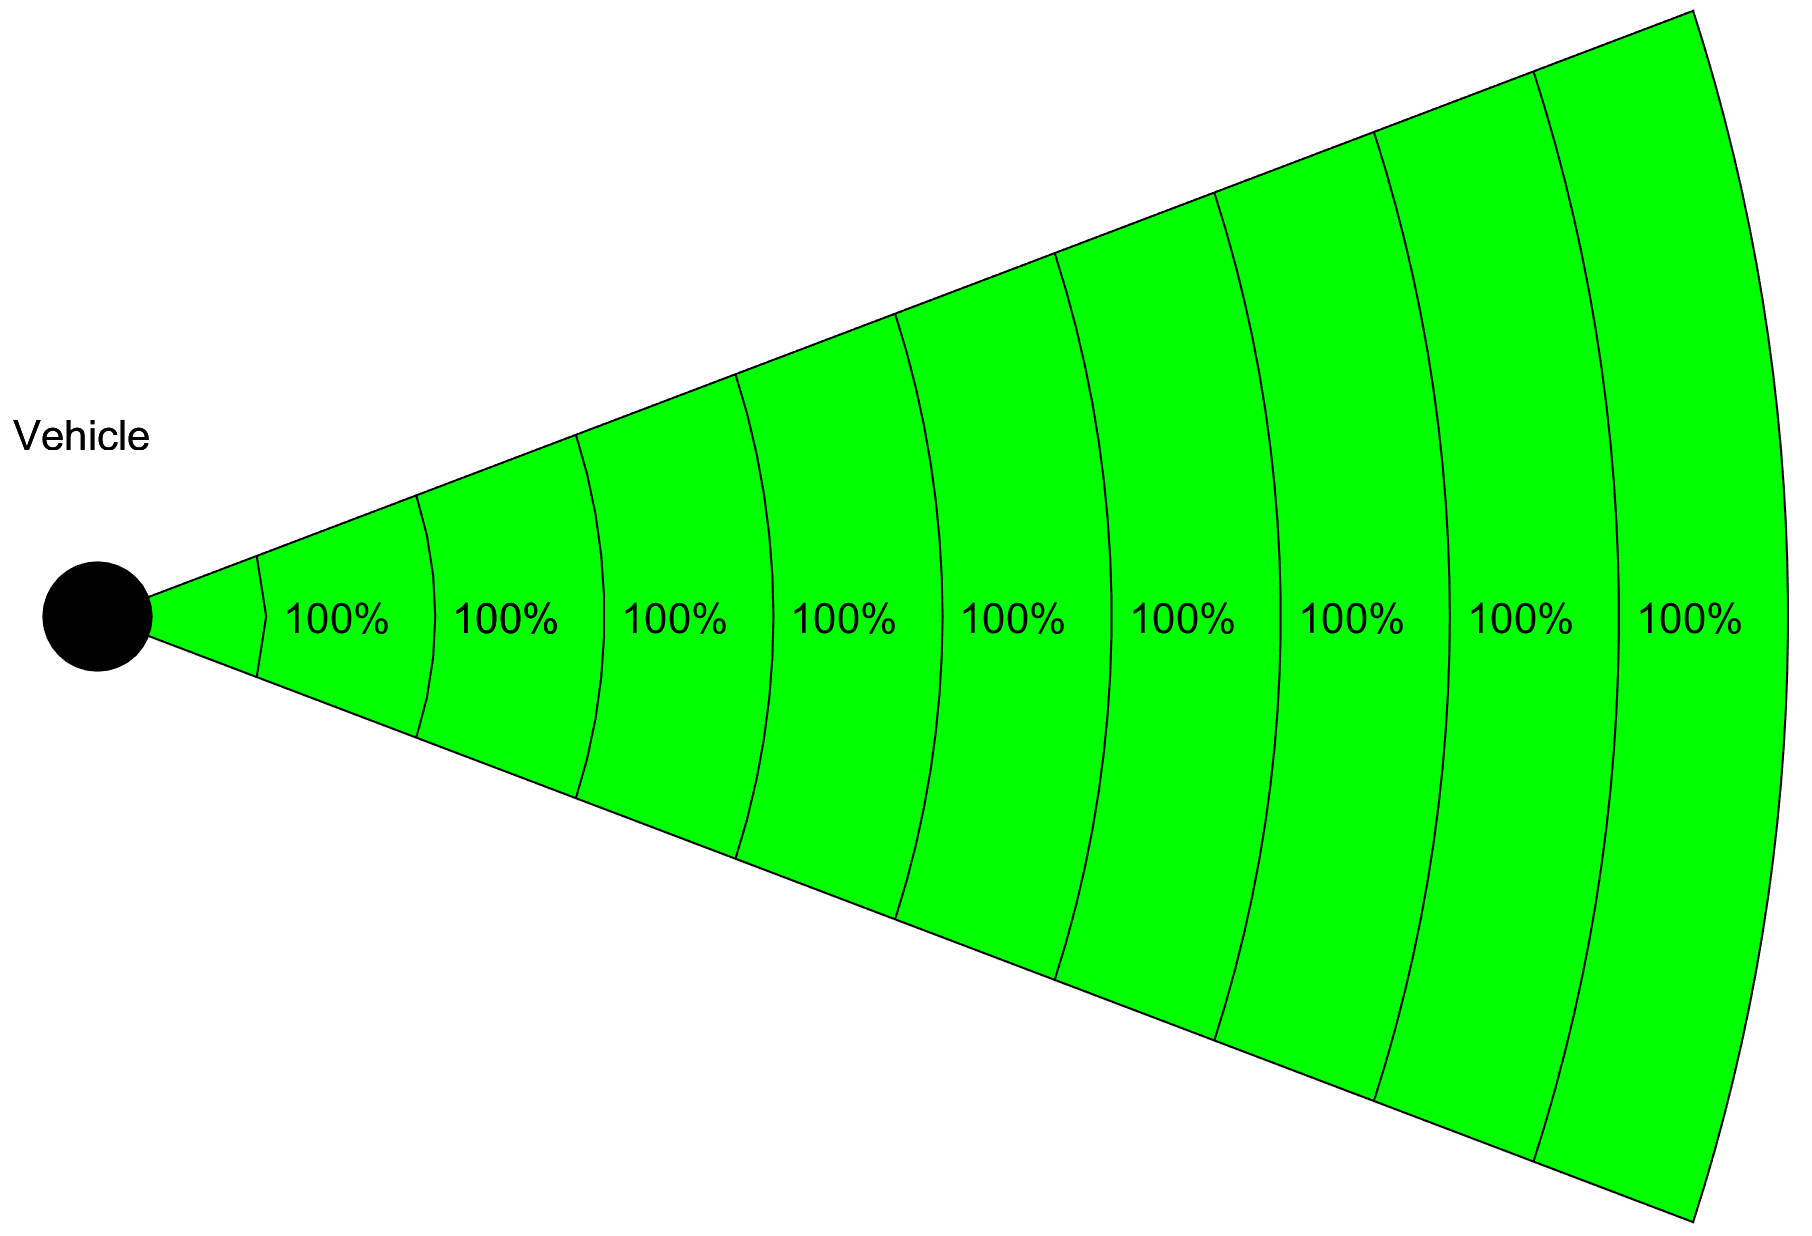
\includegraphics[width=0.7\textwidth]{\FIGDIR/P24VisibilityFreeSpace}
    \caption{Visibility probability for cell row - free space}
    \label{fig:P24VisibilityFreeSpace}
\end{figure}

\noindent The vehicle is detecting in avoidance grid $\mathscr{A}(t_1)$ and detects one obstacle $O_1$ (fig. \ref{fig:P25VisibilityFirstObstacle}). The obstacle is placed in third cell from vehicle. Note that visibility of third cell is 100 percent, because no prior hindrance in line of sight exist. 
\begin{figure}[H]
    \centering
    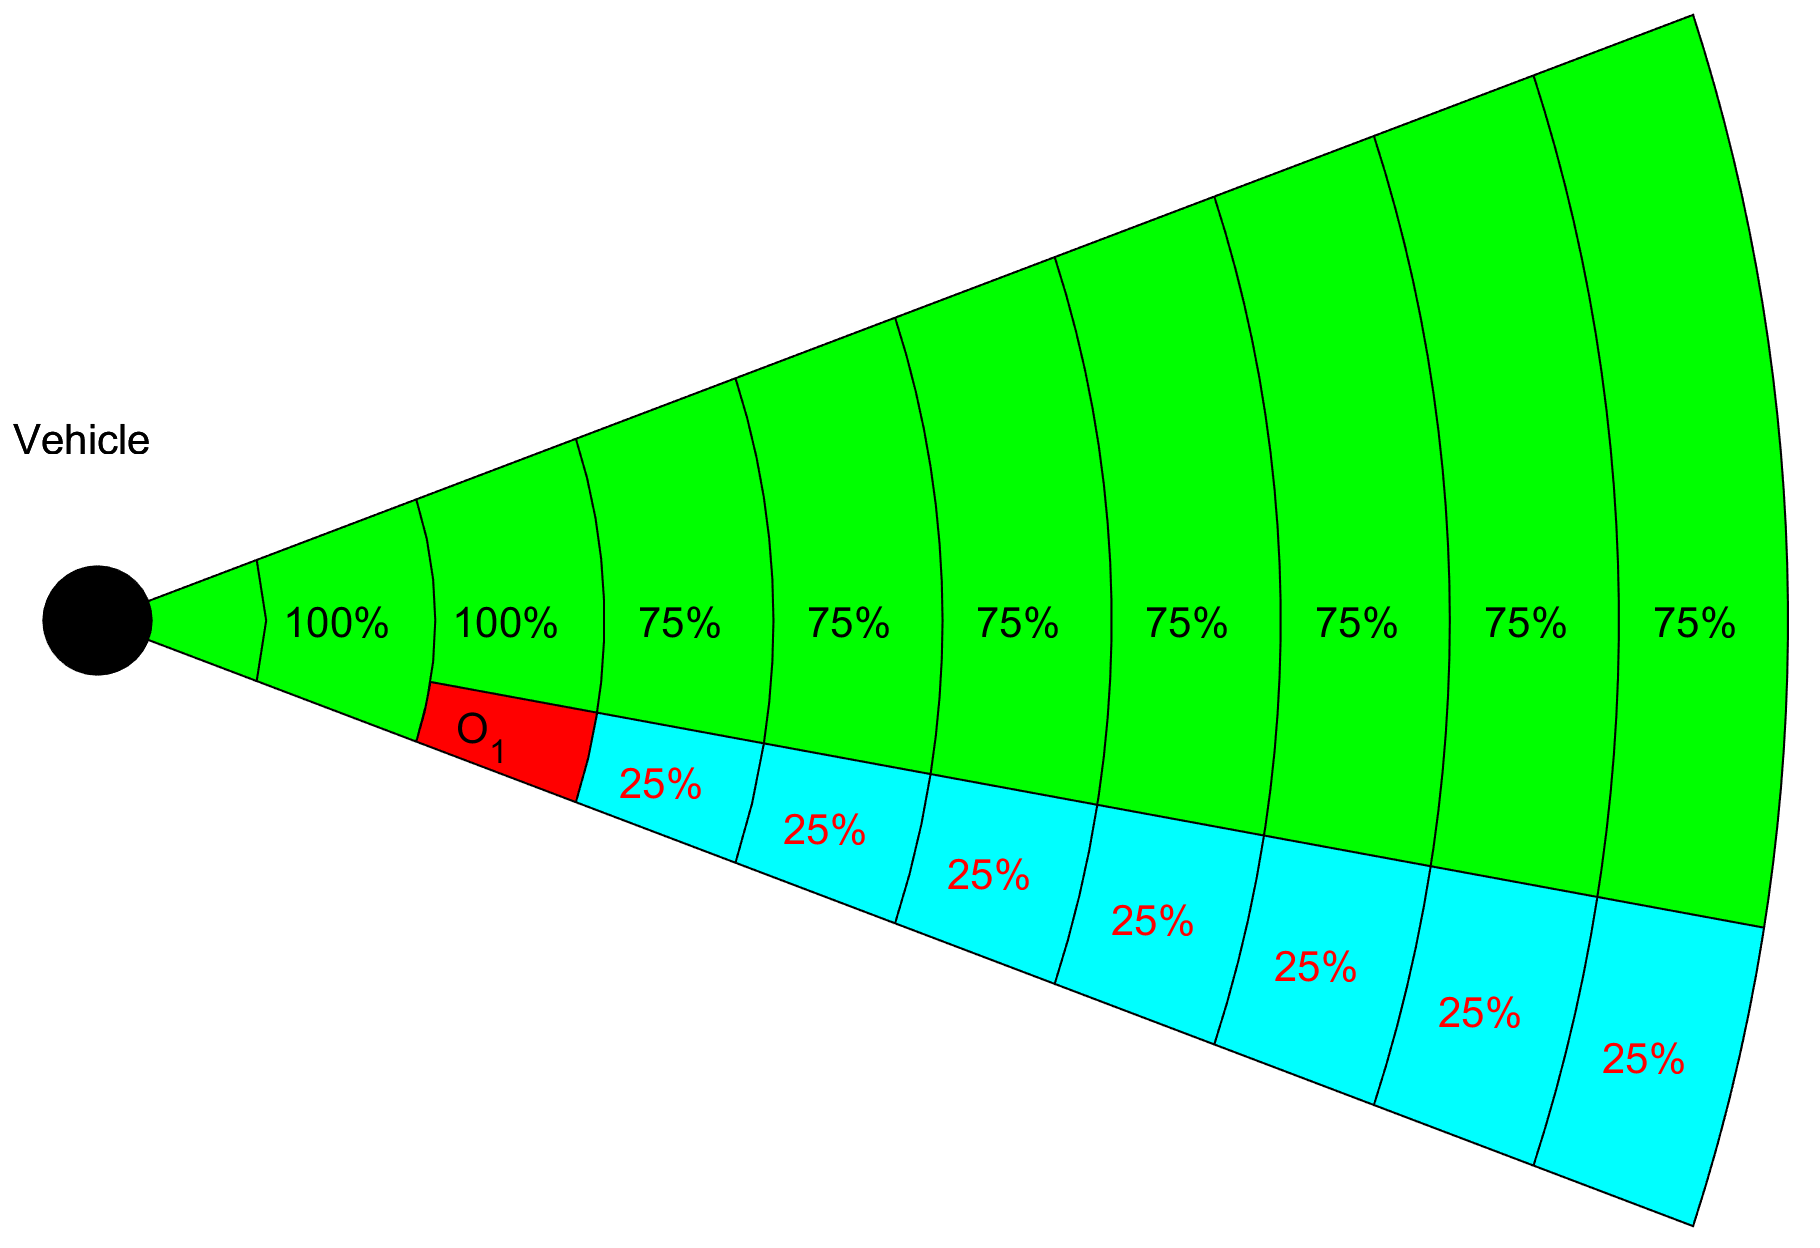
\includegraphics[width=0.7\textwidth]{\FIGDIR/P25VisibilityFirstObstacle}
    \caption{Visibility probability for cell row - first obstacle}
    \label{fig:P25VisibilityFirstObstacle}
\end{figure}

\noindent The vehicle is detecting in avoidance grid $\mathscr{A}(t_2)$ detects obstacles $O_1$, $O_2$ (fig. \ref{fig:P26VisibilitySecondObstacle}). The cell row $\mathscr{C}(j_{fix},k_{fix})$ is now  hindered with obstacles $O_1$ with hindrance $0.25$ and obstacle $O_2$ with hindrance $0.15$.
\begin{figure}[H]
    \centering
    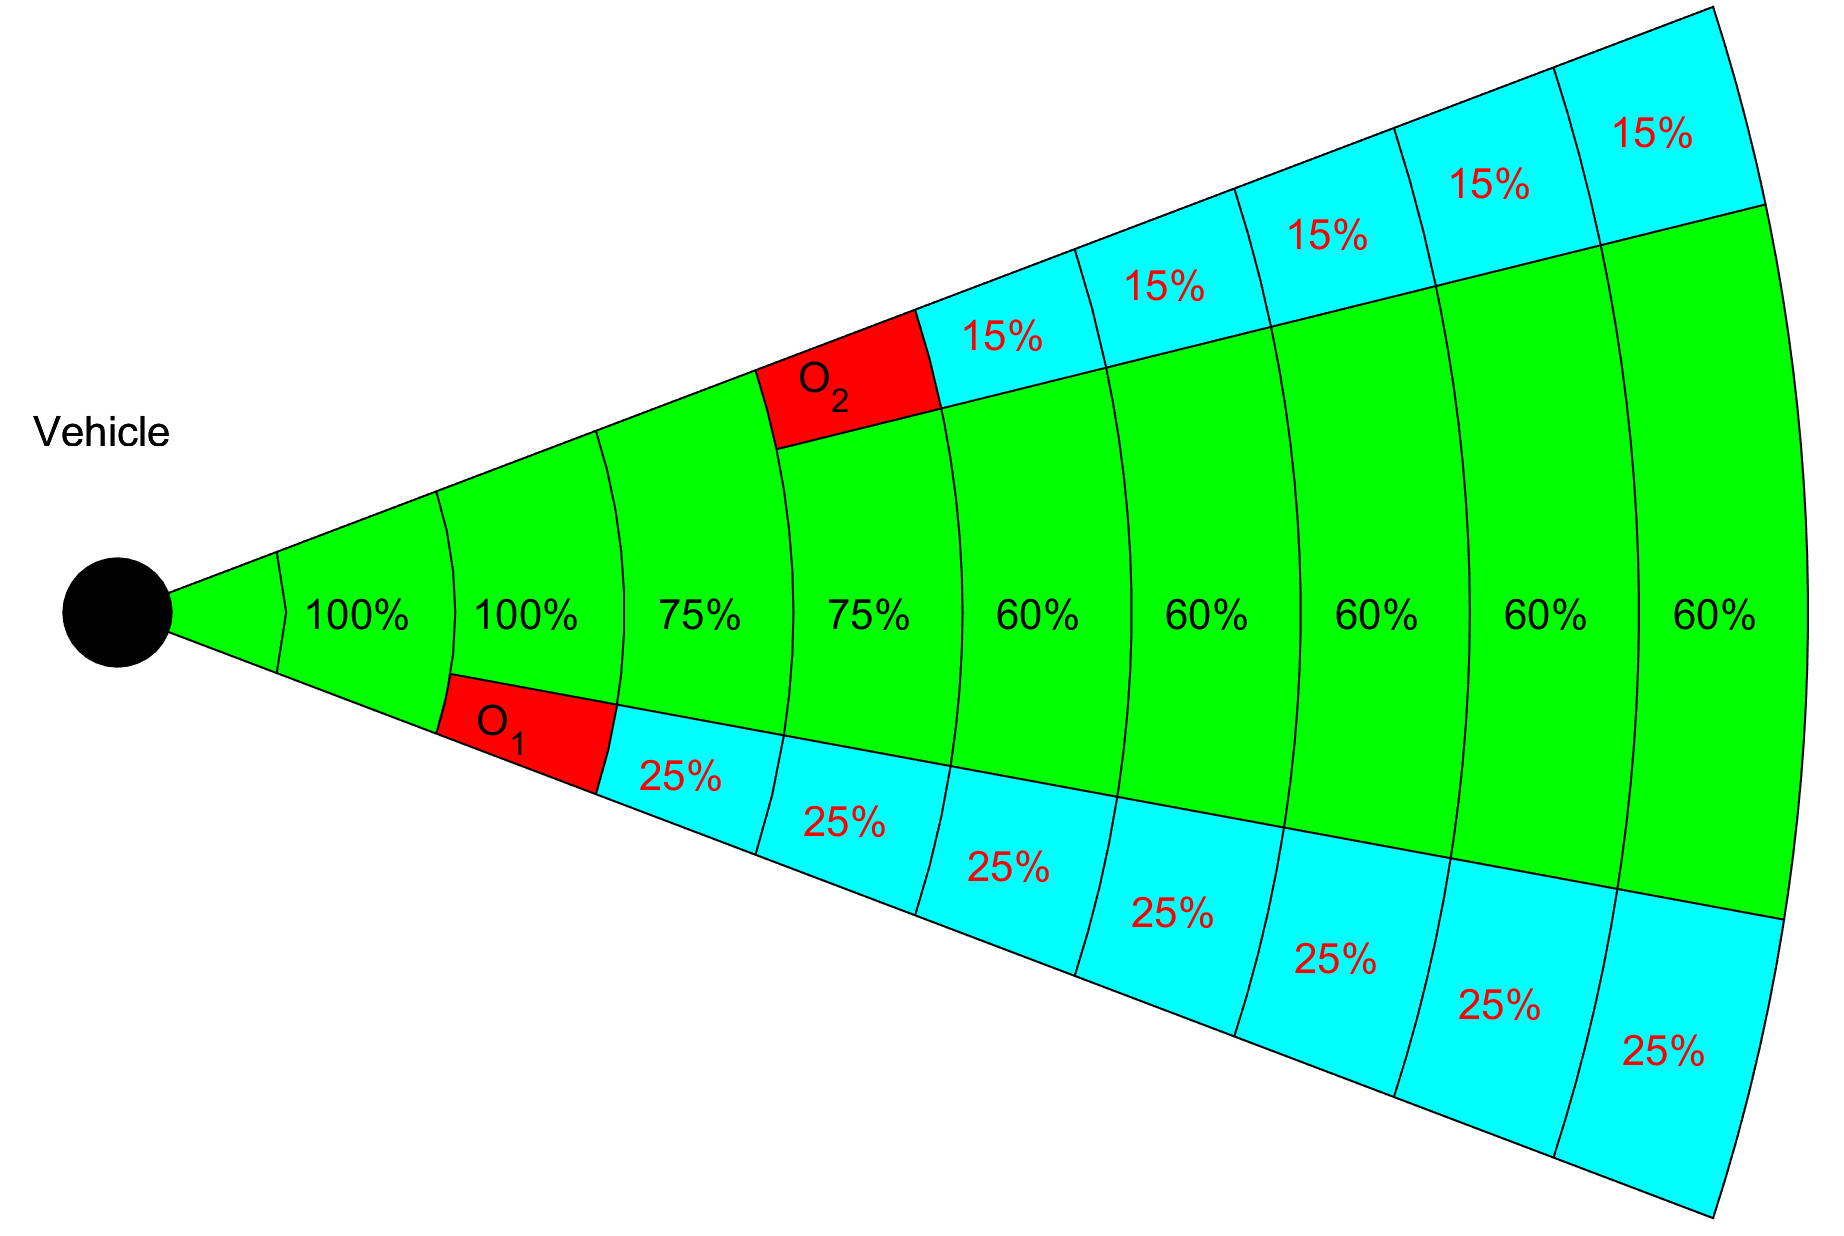
\includegraphics[width=0.7\textwidth]{\FIGDIR/P26VisibilitySecondObstacle}
    \caption{Visibility probability for cell row - second obstacle}
    \label{fig:P26VisibilitySecondObstacle}
\end{figure}

\noindent The vehicle is detecting in avoidance grid $\mathscr{A}(t_3)$ detects obstacles $O_1$, $O_2$, $O_3$ (fig. \ref{fig:P27VisibilityThirdObstacle}). The cell row $\mathscr{C}(j_{fix},k_{fix})$ is now  hindered with obstacles $O_1$ with hindrance $0.25$, obstacle $O_2$ with hindrance $0.15$, and obstacle $O_3$ with hindrance $0.20$.
\begin{figure}[H]
    \centering
    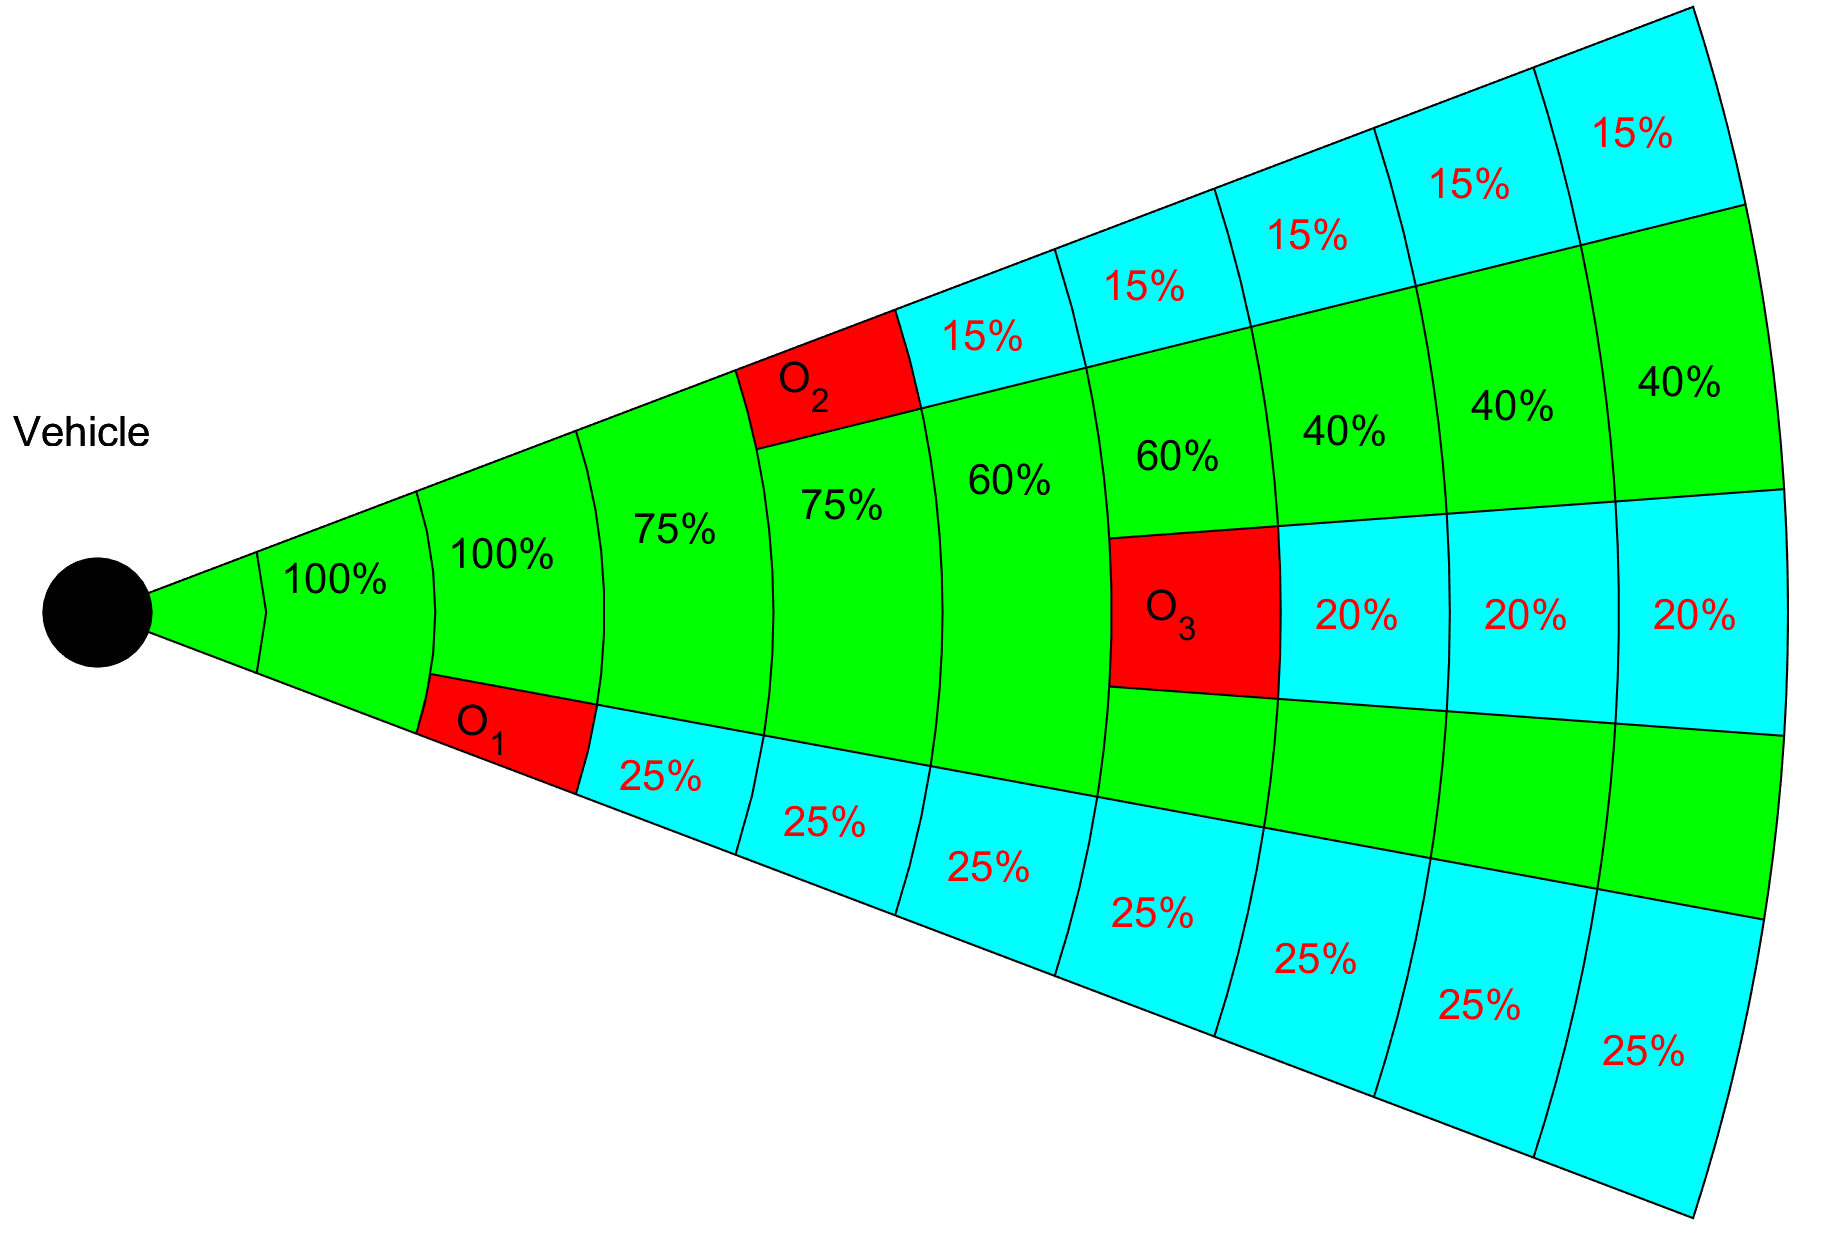
\includegraphics[width=0.7\textwidth]{\FIGDIR/P27VisibilityThirdObstacle}
    \caption{Visibility probability for cell row - third obstacle}
    \label{fig:P27VisibilityThirdObstacle}
\end{figure}

\section{Map obstacle probability}\label{sec:mapObstacleProbability}
\noindent\emph{Probability of Map Obstacle} $P_{O_M}$ occurrence follows very simple logic. There are three possible cases:

\noindent\emph{Map obstacle $O_M$} is charted on map (fig. \ref{fig:P28MapObstacleUndetected}), but is undetected by any sensor in sensor set $\mathscr{S}$. Therefore the probability of map obstacle occurrence is equal to $0$.
\begin{figure}[H]
    \centering
    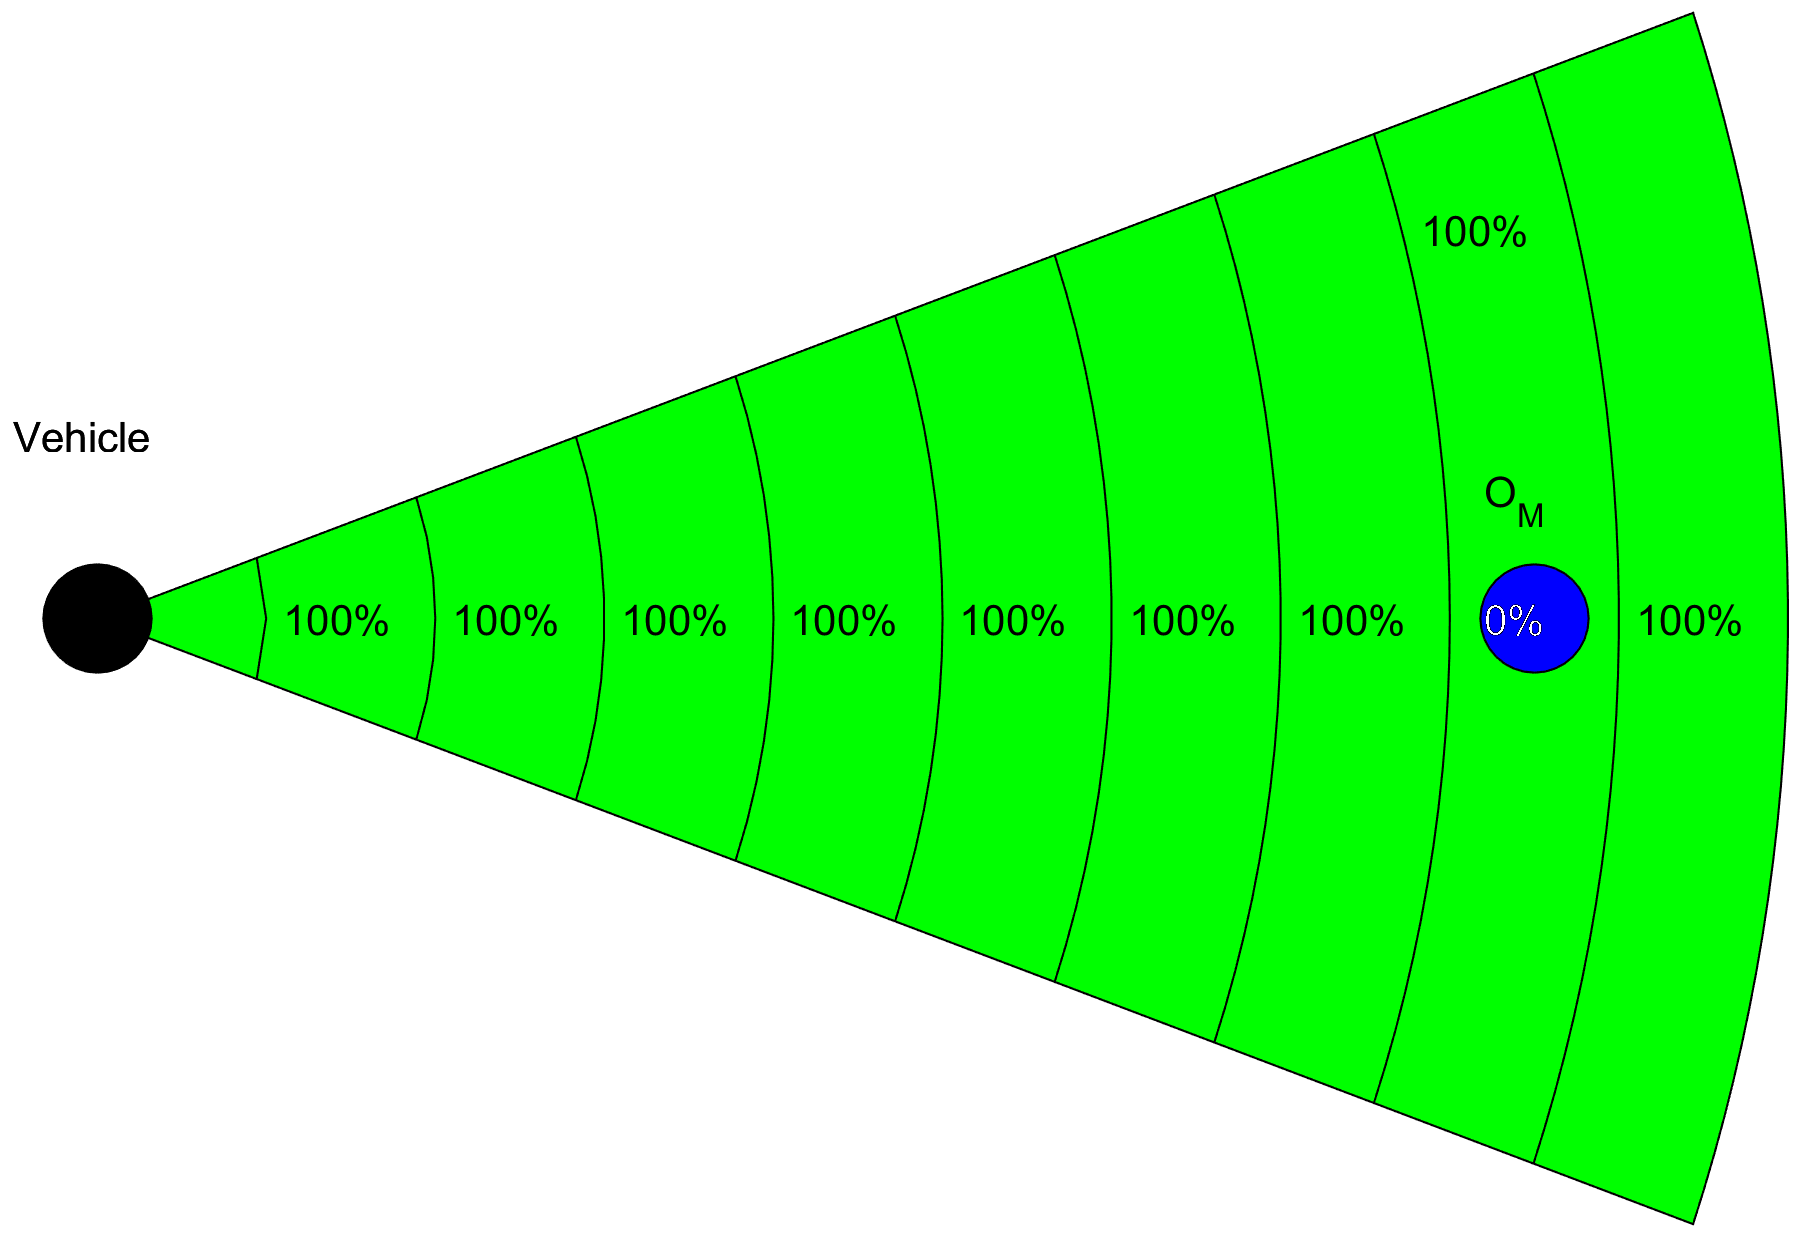
\includegraphics[width=0.7\textwidth]{\FIGDIR/P28MapObstacleUndetected}
    \caption{Map obstacle - undetected by sensory system}
    \label{fig:P28MapObstacleUndetected}
\end{figure}

\noindent\emph{Map obstacle $O_M$} is charted on map and detected by any sensor in sensor system $\mathscr{S}$ (fig. \ref{fig:P29MapObstacleDetected}). The probability of map obstacle $P_{O_M}$ is equal to probability of detected obstacle $P_{O_D}$, therefore its equal to $1$.

\begin{figure}[H]
    \centering
    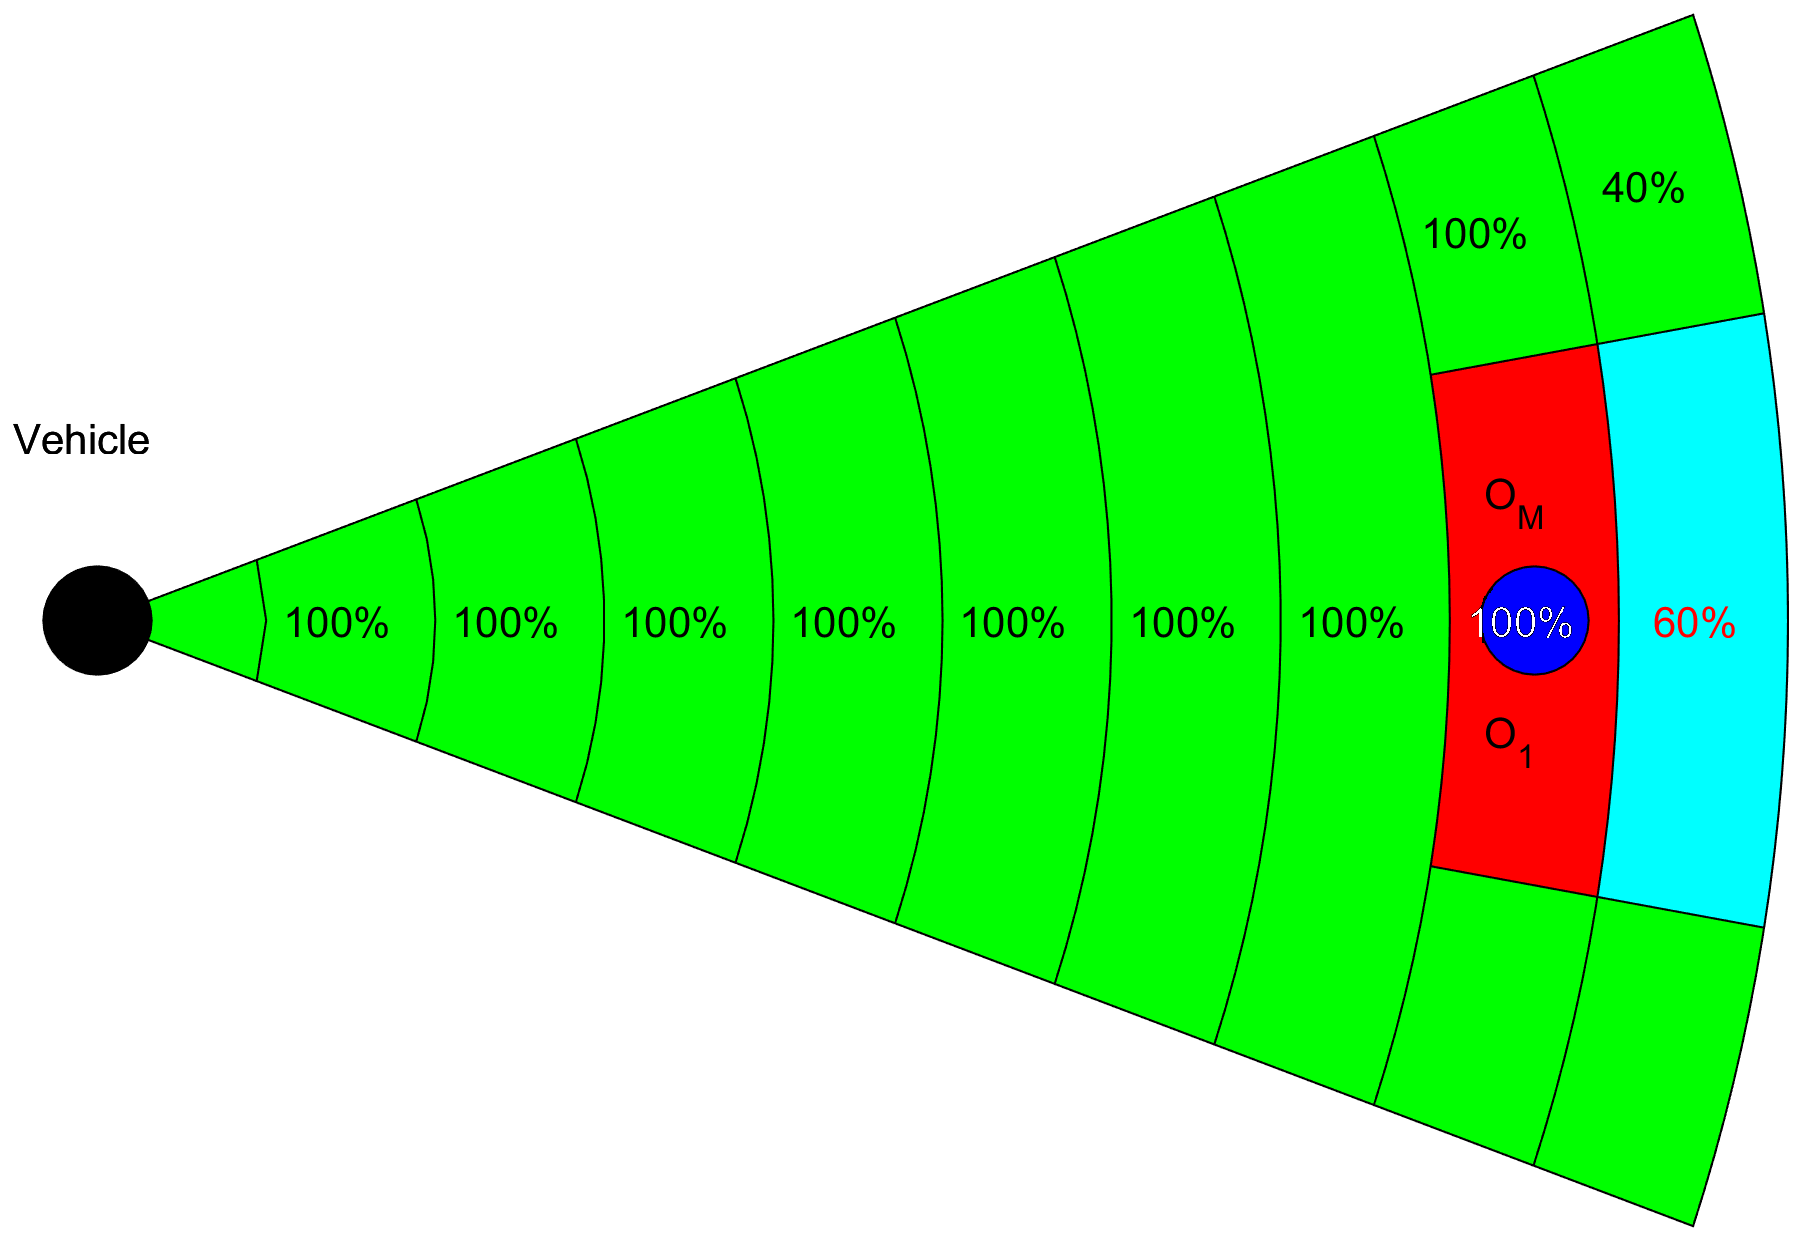
\includegraphics[width=0.7\textwidth]{\FIGDIR/P29MapObstacleDetected}
    \caption{Map obstacle - detected by sensory system}
    \label{fig:P29MapObstacleDetected}
\end{figure}

\noindent\emph{Map obstacle $O_M$} is hindered behind other detected obstacle $O_1$ (fig. \ref{fig:P30MapObstacleHiden}). The detected obstacle $O_1\in\mathscr{O}_D$ is in cell $c_{i,j,k}$ and is reducing visibility in follow up cells $c_{i_f>i,j,k}$ by $60$ percent.
\begin{figure}[H]
    \centering
    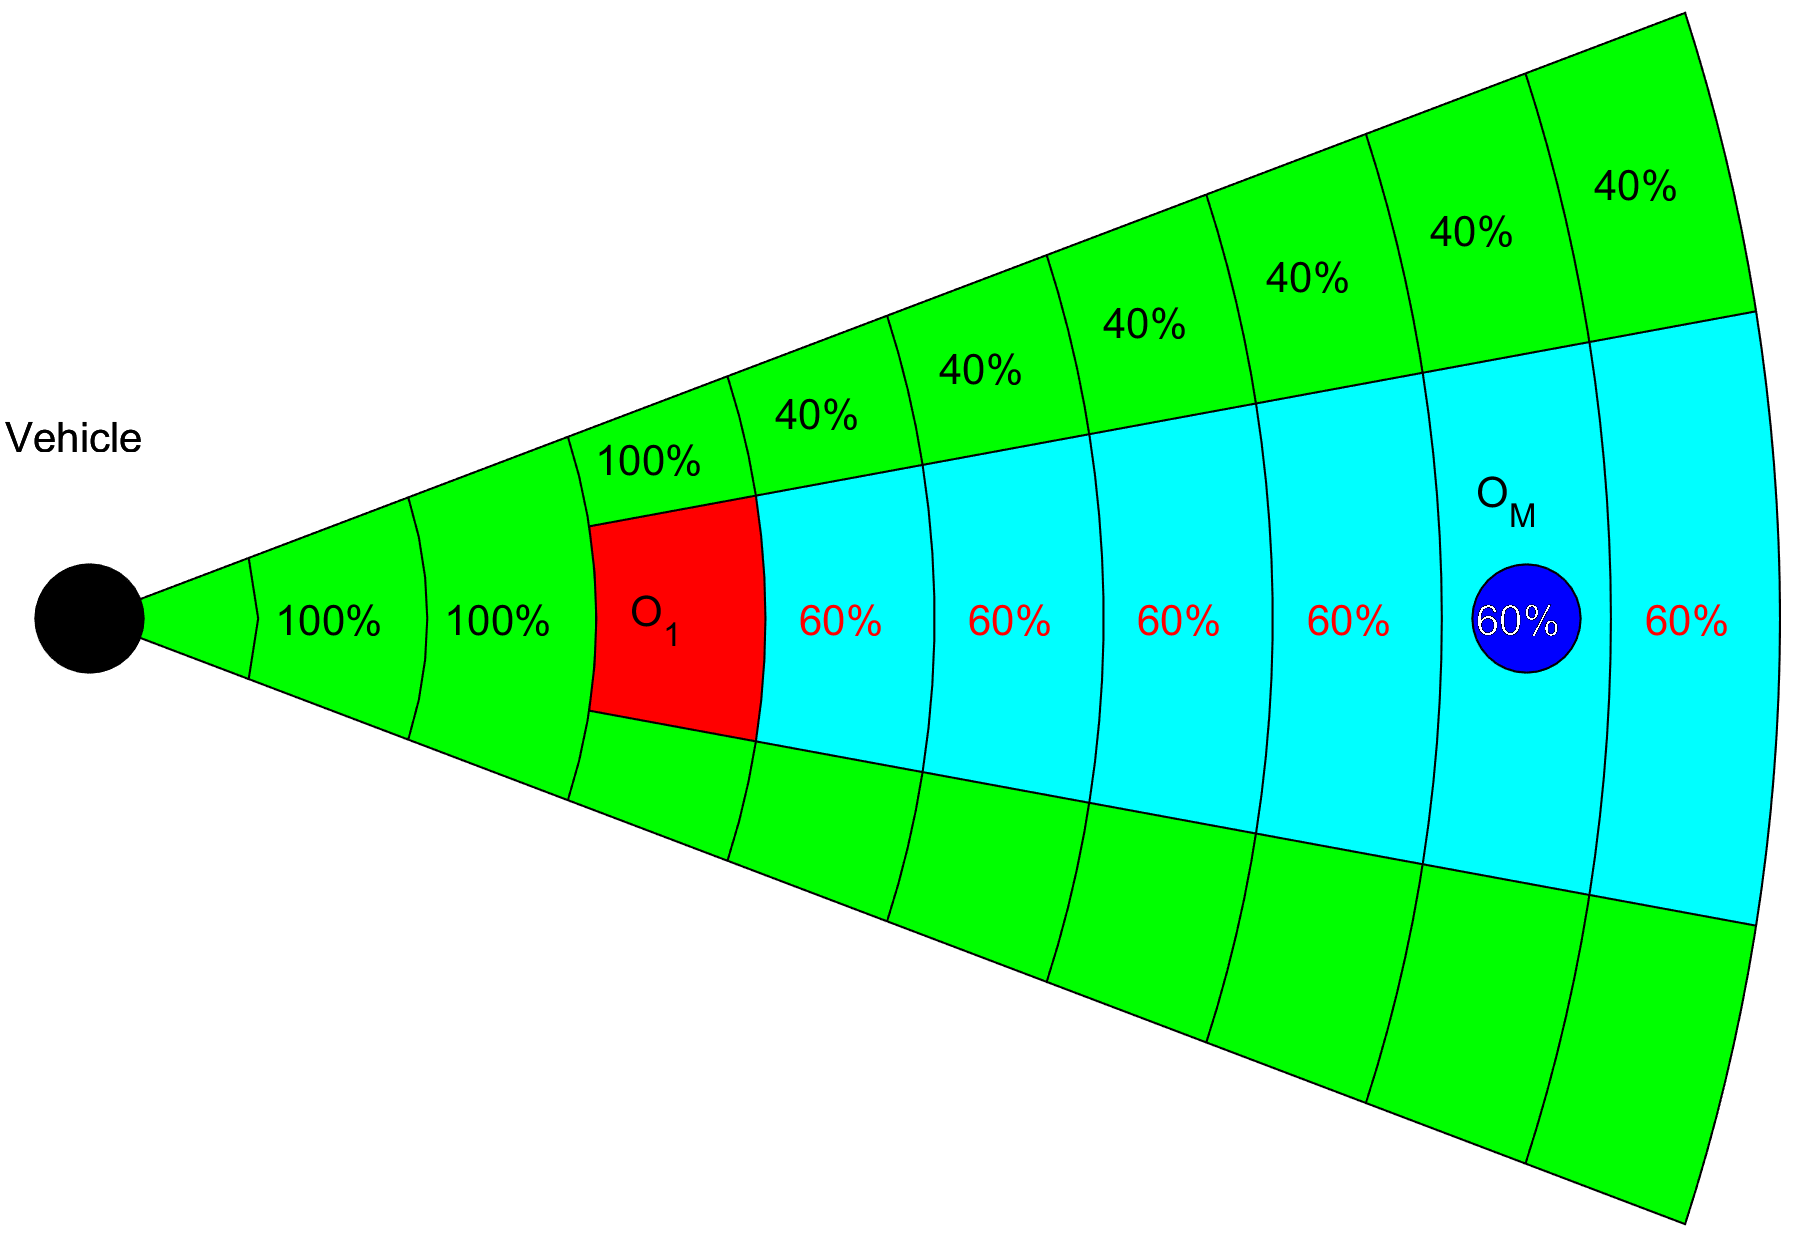
\includegraphics[width=0.7\textwidth]{\FIGDIR/P30MapObstacleHiden}
    \caption{Map obstacle - hidden behind detected obstacle}
    \label{fig:P30MapObstacleHiden}
\end{figure}

\noindent\emph{The formulation of final map obstacle probability} $P_{O_M}(c_{i,j,k})$ is given by previous examples which are giving the \emph{desired behaviour}. First we start with obstacle map definition.

The obstacle map $\mathscr{O}_m$ (\ref{eq:obstacleMap}) defines an map obstacle set $o=[\vec{p},\vec{o},r,\vec{a}]$ where $\vec{p}$ is position in global coordinate frame (center of mass), $\vec{o}$ is orientation bounded to global coordinate reference frame, $r$ is offset radius and $a$ is set pf additional parameters.
\begin{equation}\label{eq:obstacleMap}
    \mathscr{O}_M= \left\{[\vec{p},\vec{o},r,\vec{a}]:\vec{p}\in\R^3, \vec{o}\in\R^3, r\in (0,\infty),\vec{a}\in\R^k,k\in\N\right\}
\end{equation}

The space covered by any obstacle $o\to\R3$ is non-empty by definition. There are following types of charted obstacle considered in this example.

\begin{enumerate}
    \item\emph{Ball obstacle $\vec{a}=\varnothing$} - simple ball with center at $\vec{p}$, with offset radius $r$.
    \item\emph{Line obstacle $\vec{a}=[l]$} - simple line defined by length $l\in(0,\infty)$ with center at $\vec{p}$ and given orientation $\vec{o}$ with respect to main axis in global coordinate frame, with offset radius $r$.
    \item\emph{Plane obstacle $\vec{a}=[l,w]$} - bounded rectangle plane partition defined by length $l\in(0,\infty)$, and width $w\in(0,\infty)$ with center at $\vec{p}$ and given orientation $\vec{o}$ with respect to main axis in global coordinate frame, with offset radius $r$.
    \item\emph{Cuboid obstacle $\vec{a}=[l,w,d]$} - bounded cuboid space partition defined by length $l\in(0,\infty)$, width $w\in(0,\infty)$, and depth $d\in(0,\infty)$ with center at $\vec{p}$ and given orientation $\vec{o}$ with respect to main axis in global coordinate frame, with offset radius $r$.
\end{enumerate}
\noindent The obstacle set for some grid $\mathscr{A}$ at decision time $t_i$ intersection with obstacle map $\mathscr{O}_m$ is given by $\mathscr{O}_M(\mathscr{A}(t_i))$ (\ref{eq:obstacleMapAvoidanceGridIntersection}). Where map obstacle space $o$ is projected into avoidance grid space $\mathscr{A}(t_i)$. Projection output $\vec{p}_l\subset\R^3$ is partial subset of local coordinate frame space given by $A(t_i)$. If there exist non empty intersection between avoidance grid $\mathscr{A}(t_i)$ and local projection of obstacle space $\vec{p}_l$ then the given obstacle belongs to $\mathscr{O}_M(\mathscr{A}(t_i))$.

\begin{equation}\label{eq:obstacleMapAvoidanceGridIntersection}
    \mathscr{O}_M(\mathscr{A}(t_i))=\left\{o\in\mathscr{O}_M:\vec{p}_l:o \to\mathscr{A} (t_i), \vec{p}_l \cap \mathscr{A}(t_i)\neq\varnothing \right\}    
\end{equation}

\noindent $\mathscr{O}_M(c_{i,j,k},\mathscr{A}(t_i))$ (\ref{eq:obstacleMapCellSapceIntersection}) is analogy to $\mathscr{O}_M(\mathscr{A}(t_i))$ (\ref{eq:obstacleMapAvoidanceGridIntersection}). The cell space $c_{i,j,k}\subset\mathscr{A}(t_i)$ is considered as criterion instead of avoidance grid $\mathscr{A}(t_i)$. $\mathscr{O}_M(c_{i,j,k},\mathscr{A}(t_i))$ represents set of map obstacles in cell $c_{i,j,k}$ in context of acoidance grid $\mathscr{A}(t_i)$.

\begin{equation}\label{eq:obstacleMapCellSapceIntersection}
    \mathscr{O}_M(c_{i,j,k},\mathscr{A}(t_i))=\left\{o\in\mathscr{O}_M:\vec{p}_l:o \to\mathscr{A} (t_i), \vec{p}_l \cap c_{i,j,k} \neq \varnothing \right\}    
\end{equation}

\noindent\emph{Base probability of map obstacle} $P_{O_M,B}$ for single map obstacle $o\in\mathscr{O}_M$ (\ref{eq:baseProbabilityMapObstacleInCell}) is given as ration between intersection volume $\iiint (o\to\mathscr{A}(t_i))\cap c_{i,j,k} \quad \text{d}x\text{d}y\text{d}z$ and cell volume $\iiint c_{i,j,k}\quad\text{d}x\text{d}y\text{d}z$

\begin{equation}\label{eq:baseProbabilityMapObstacleInCell}
    P_{O_M,B}(o,c_{i,j,k}) = \frac{\iiint (o\to\mathscr{A}(t_i))\cap c_{i,j,k} \quad \text{d}x\text{d}y\text{d}z}{\iiint c_{i,j,k}\quad\text{d}x\text{d}y\text{d}z}
\end{equation}

\noindent\emph{Base probability of map obstacle} $P_{O_M,B}$ for map obstacle set  $\mathscr{O}_M$ (\ref{eq:baseProbabilityMapObstacleSetInCell}) is calculated in similar manner as base probability of map obstacle $P_{O_M,B}$ for single map obstacle $o\in\mathscr{O}_M$ (\ref{eq:baseProbabilityMapObstacleInCell}). The obstacle member of denominator has changed to space union of all obstacle space in local coordinate frame of avoidance grid $\mathscr{A}(t_i)$ as follow $\bigcup_{o\in\mathscr{O}_M}o\to\mathscr{A}(t_i)$.
\begin{equation}\label{eq:baseProbabilityMapObstacleSetInCell}
    P_{O_M,B}(\mathscr{O}_M,c_{i,j,k}) = \frac{\iiint \left(\bigcup_{o\in\mathscr{O}_M}o\to\mathscr{A}(t_i)\right) \cap c_{i,j,k} \quad \text{d}x\text{d}y\text{d}z}{\iiint c_{i,j,k}\quad\text{d}x\text{d}y\text{d}z}
\end{equation}

\noindent\emph{Final map obstacle probability} $P_{O_M}(c_{i,j,k})$ (\ref{eq:finalMapObstacleProbability}) is given as product of \emph{base probability of map obstacle} $P_{O_M,B}$ for map obstacle set  $\mathscr{O}_M$ (\ref{eq:baseProbabilityMapObstacleSetInCell}), and inverted \emph{final visibility probability $P_V(c_{i,j,k})$} (\ref{eq:FinalVisibilityProbability}). 
\begin{equation}\label{eq:finalMapObstacleProbability}
    P_{O_M}(c_{i,j,k})=P_{O_M,B}(\mathscr{O}_M,c_{i,j,k})\quad(\ref{eq:baseProbabilityMapObstacleSetInCell})\times\left(1-P_{V}(c_{i_c,j_c,k_c},\mathscr{S})\quad(\ref{eq:FinalVisibilityProbability})\right)
\end{equation}